\documentclass[11pt]{article}

% Related to page geomety
\usepackage[a4paper,vmargin={2.4cm,2.8cm},hmargin={2.4cm,2.4cm}]{geometry}
\usepackage[utf8]{inputenc}
\usepackage{fancyhdr}
\pagestyle{fancy}
\renewcommand{\headrulewidth}{1pt}
\fancyhead[C]{CONFIDENTIAL}
\fancyhead[L]{Team 04 - Contour Detection}
\fancyhead[R]{M2DS Capstone projects, IPP, 2025}


% Related to math
\usepackage{amsmath,amssymb,amsfonts,amsthm}

% Related to figures
\usepackage{graphicx}

%Related to referencing
\usepackage{hyperref}
\usepackage{cleveref}

% =============================================================================
% Document
% =============================================================================
\title{Captone Project Report Vinci - Contour Detection}
\author{Fabien Lagnieu, Maha Kadraoui, Tristan Waddington, Abdoul Zeba}
\date{20/03/2025}
\begin{document}

\begin{center}
\textbf{Contour detection} \\
Fabien Lagnieu, Maha Kadraoui, Tristan Waddington, Abdoul Zeba\\
\textbf{Mentor:} Stéphane Maviel (CEO Vinci/Diane\footnote{Diane is Vinci's inside Startup tasked to find numerical solutions
to ease the work of Vinci collaborators.}) \\\vspace{2em}
\textbf{\Large }
\end{center}
\vspace{-1cm}

Architects are drawing floor plans using a Computer-Aided Design (CAD) software. These files are used
by engineers to plan and conduct the construction of the building. In this process,
additional measures are needed such as the room size or adjacency. \textbf{The goal of 
this project is to develop a tool that can automatically detect the contours of 
the rooms in the floor plan to draw it back into the CAD software.}

% This is a latex template for your report. Your report should fit in 5 pages  excluding references and appendices and summarize your main findings and process of thoughts. It should be self-contained, and you should not modify the template. . You can use appendices for additional figures and details, provide explanation of parallel tracks you gave up etc.
\begin{figure}[h]
    \centering
    
\includegraphics[width=0.1\textwidth]{figures/Diane.png}
    \hspace{0.1\textwidth}
    
\includegraphics[width=0.3\textwidth]{figures/logo_vinci.png}
    \hspace{0.1\textwidth}
    
\includegraphics[width=0.1\textwidth]{figures/ipparis.png}

    %\caption{Example figure with example spacing and caption: Left, ipp paris logo. Right, ipp paris logo.}
    \label{fig:my_label}
\end{figure}

% =============================================================================
% Section context
% =============================================================================

\section{Context}
Vinci's engineers are dealing with a different floor plan for every project they are working on.
Every plan has its own drawing style and the contours of the rooms are often mixed with other
lines, but they need this information to plan the location of smoke detectors, fire extinguishers,
and other facilities in the building. The goal of this project is to develop a tool that can
automatically detect the contours of the rooms in the floor plan and draw back the polygons in the CAD software as 
a vector layer for further automatic processing. 
Diane's teams have already worked on this problem and developed a first version of the tool
that is too slow and not accurate enough. They are looking for other approaches
to improve it.
% \textit{What is the question to be answered? Why is it important for the mentor?\\
% Present briefly the dataset (type of data, dimensionality, what else is notable?)}

\paragraph{Datasets}
We are given examples of GeoJSON\footnote{The current standard for GeoJSON format was 
published in August 2016 by the Internet Engineering Task Force (IETF), 
in \href{https://datatracker.ietf.org/doc/html/rfc7946}{RFC 7946}.} exports of CAD plans. The first dataset is 
composed of 9 GeoJSON exports of floor plans from very different buildings (datacenter, 
hospital, car-park ...). Each file contains a list of points 
connected together to form lines or polygons representing walls, windows, doors, 
or even furniture.

The second dataset exports the floor plans of 5 whole buildings in the same format
as the previous one. Each plan is joined by a second file 
containing the actual contours of the rooms as a target. This dataset is really useful 
to compute metrics of our models.

% =============================================================================
% Section methods
% =============================================================================

\section{Methods}
\label{sec:methods}

% \textit{Which methods did you try or could you have tried?\\
% Which one did you choose and why?}\\\\
% Include references if you use a non-standard method \cite{pml1Book}. The corresponding entry is defined in the file \texttt{references.bib}. Do no cite textbooks, \cite{pml1Book} is just an example. 
After a first phase of data cleaning we focus on two different paths to solve the problem:

\begin{enumerate}
    \item \textbf{Geometric process} Transform the geometries into normalized segments 
    \cite{Schafer2011AutomaticGO} then cluster the lines to 
    create the polygons\cite{dominguez2012Semiautomaticdetection} of the contours. This path relies on the
    geometric libraries \texttt{shapely} and \texttt{geopandas}. The graph representation 
    was later discarded as too computational expensive.
    \item \textbf{Image segmentation} Using a dense literature review\cite{PIZARRO2022104348}, we 
    spot some successful uses of CNNs\cite{ijgi10020097}. This same paper also provides the list
    of datasets of floor plans as images we can use for training deep learning models.
    Ultimately, this path gives us the idea of the segmentation of the floor plans 
    into rooms, using basic computer vision methods and the Segment 
    Anything Model (SAM)\cite{kirillov2023segment}.
\end{enumerate}

\textbf{At the end of our research, we produce 3 models of different complexity
ranging from geometric hand-crafted rules to fully automatic computer vision:}\\ 
\texttt{SegmentBasedClustering}, 
\texttt{VisionSegmentation}, 
and \texttt{SegmentAnythingModel}.\\ They share common steps and a global representation
is given in figure \ref{fig:global_pipeline}. The individual pipelines are detailed 
in the following sections.
\begin{figure}[h]
    \centering
    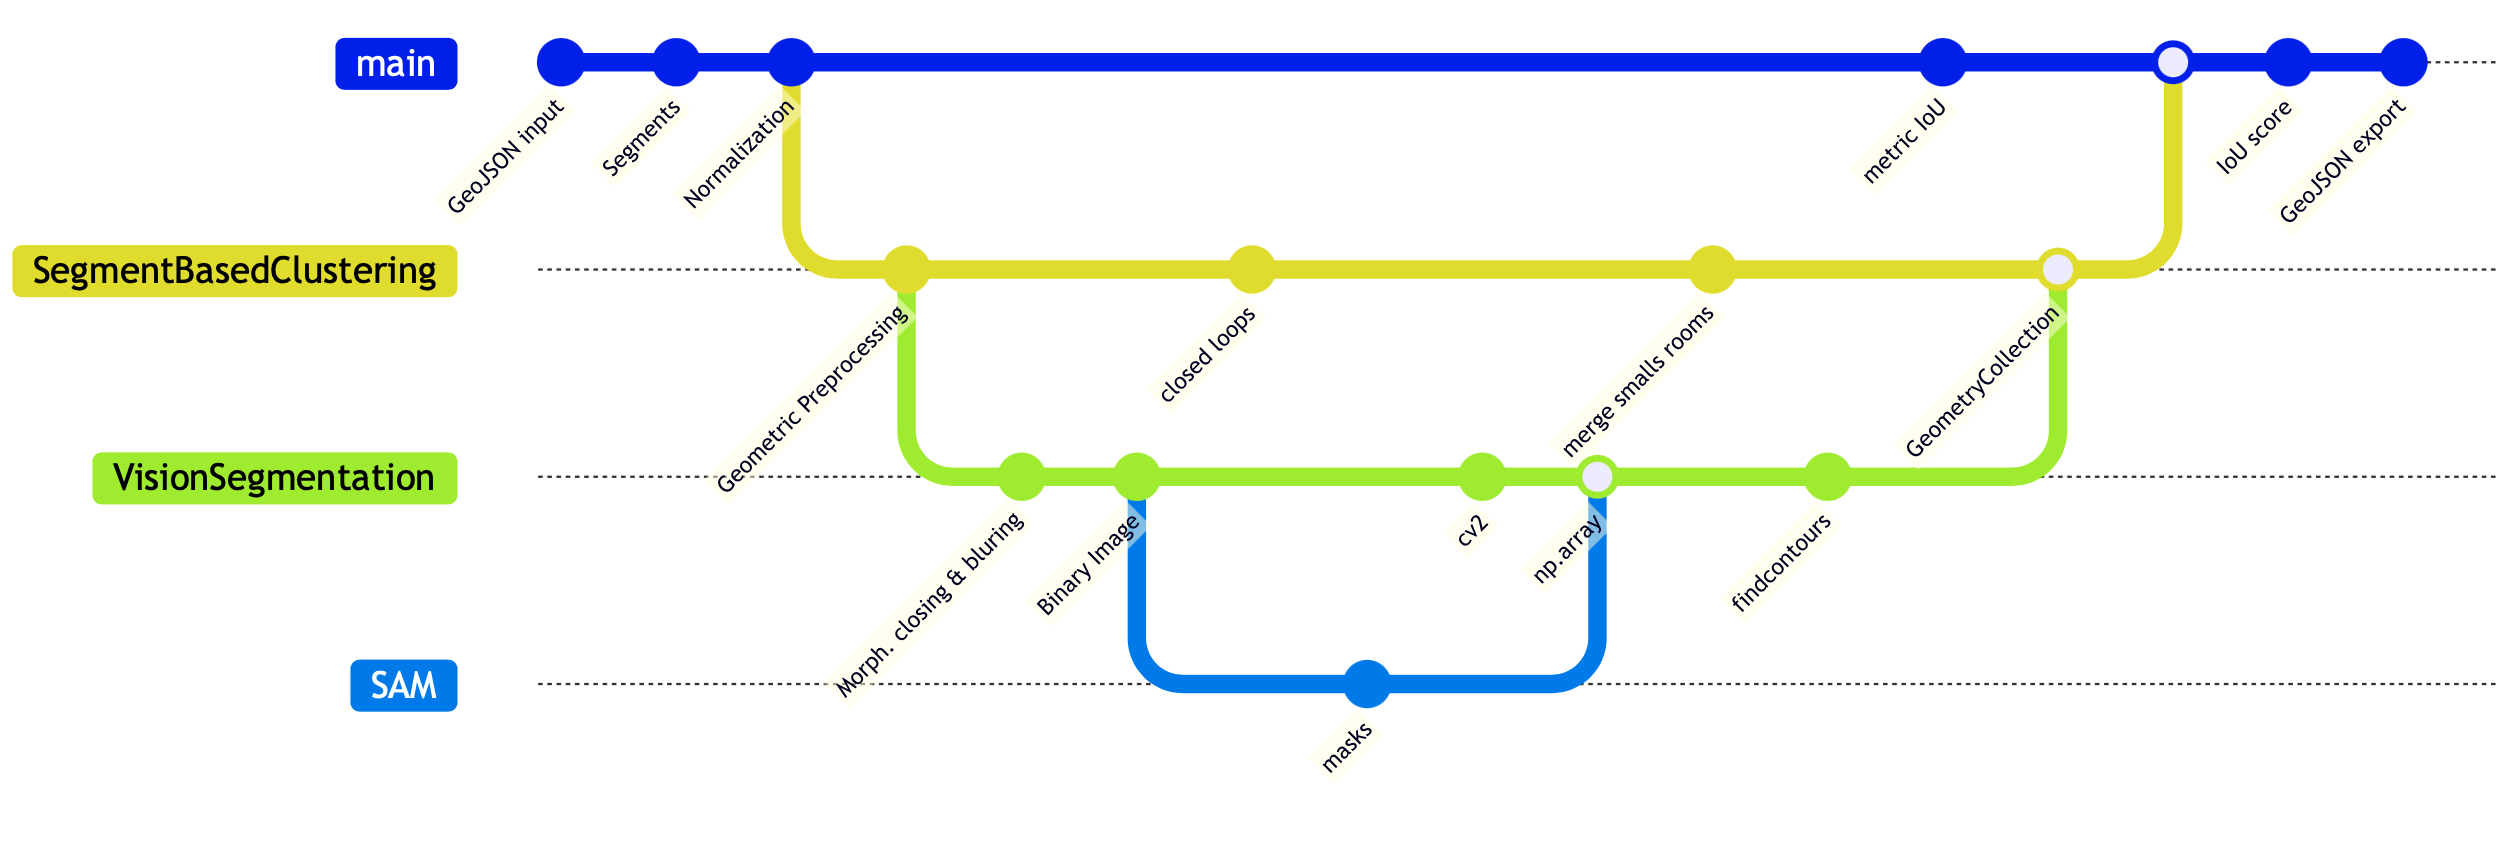
\includegraphics[width=01\linewidth]{figures/CapstoneGit.png}
    \caption{Articulation of the shared steps of the three models.}
    \label{fig:global_pipeline}
\end{figure}

% =============================================================================
% FM @Maha
\subsection{Geometric Preprocess}
\label{sec:geometric_preprocess}

Before feeding GeoJSON files into the model, a preprocessing step is applied to 
clean and standardize the segment data. This ensures accurate room segmentation 
while minimizing errors caused by noise, misaligned geometries and above all,
plans drawn with different scales.

\paragraph{Preprocessing Steps}
The preprocessing consists of five successive steps:
(i) \textbf{Splitting into segments} the complex geometries.
(ii) \textbf{Normalizing segments} by sorting segment endpoints to avoid duplicate representations and rescaling to the meter unit.
(iii) \textbf{Snapping} close endpoints by aligning nearby segment endpoints (within 0.05m) for better connectivity.
(iv) \textbf{Removing isolated} segments by eliminating segments not connected to any others.
(v) \textbf{Merging collinear} segments by combining nearly aligned segments to reduce fragmentation.

The preprocessing significantly reduces the number of segments (up to 70\%) while 
preserving the overall geometry. See figure \ref{fig:geojson_comparison} for visual 
results.
Additional details and tables can be found on appendix \ref{app:sec:geomdetails}.


\subsection{Model 1: \texttt{SegmentBasedClustering}, Based on Geometric Rules}

This model is a geometric rule-based method designed to extract room boundaries
from architectural floor plans provided in GeoJSON format.
This method 
leverages classic computational geometry techniques to detect closed paths
and segment parts based on structural constraints. It does not require training data.
Further details and pipeline  are described in appendix \ref{app:sec:SBCdetails}. 


\begin{figure}[h]
    \centering
    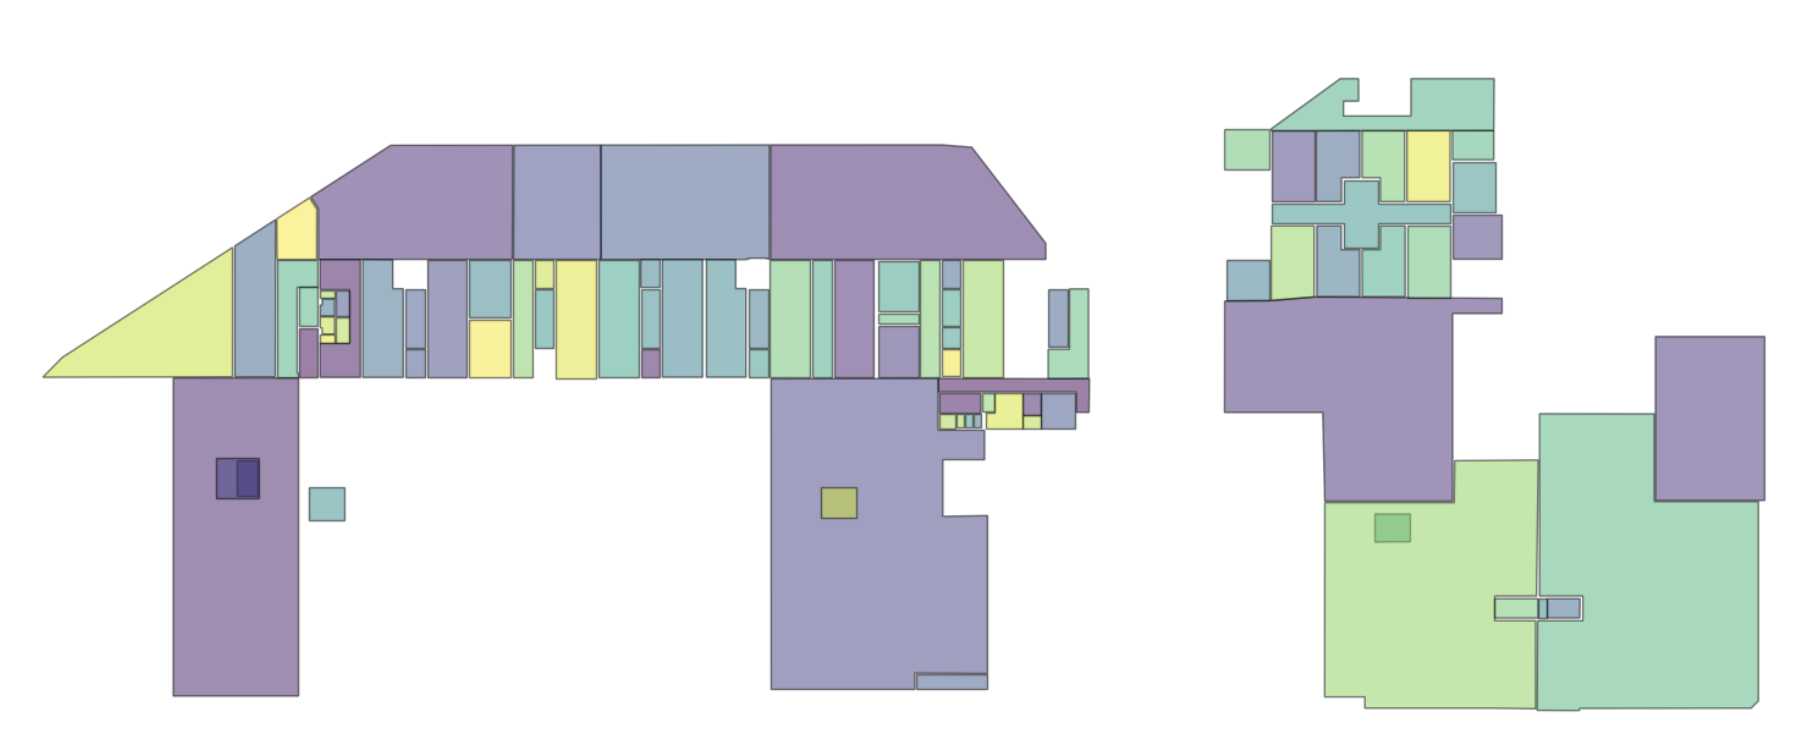
\includegraphics[width=0.6\linewidth, height=4cm, keepaspectratio]{figures/simplemodel.png}
    \caption{Example of precise rooms detections using \texttt{SegmentBasedClustering}.}
    \label{fig:closed_paths}
\end{figure}

\paragraph{Discussion} \texttt{SegmentBasedClustering} offers an efficient approach to segmenting 
rooms in architectural plans without resorting to complex models nor heavy 
computing resources. By leveraging 
topological and geometric operations, the method ensures robust room segmentation.
However, this approach needs explicit physical separations between rooms. 
If there are no walls or voids, inconsistent results may be obtained.


% =============================================================================
% FM @Fabien
\subsection{Model 2: \texttt{VisionSegmentation}, Based on Computer Vision}

The other rule-based method leverages classical computer 
vision techniques to extract room boundaries from 
geometric data, without requiring training datasets.

The pipeline consists of converting vector data into raster images, applying 
image processing operations to detect closed areas, and exporting the resulting 
room contours back into a geo-referenced vector format (GeoJSON). The entire 
workflow is based on \texttt{OpenCV} image processing primitives and geospatial data 
transformations from \texttt{shapely}. Further details and pipeline description 
can be found in appendix \ref{app:sec:CVdetails}. 

\begin{figure}[htp!]
    \centering
    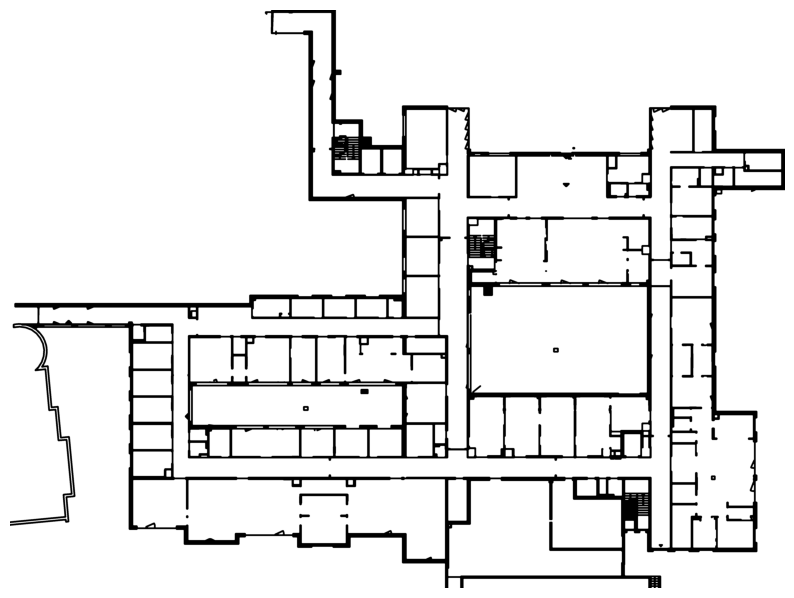
\includegraphics[width=0.48\linewidth]{figures/01.binary_image.png}
    \hfill
    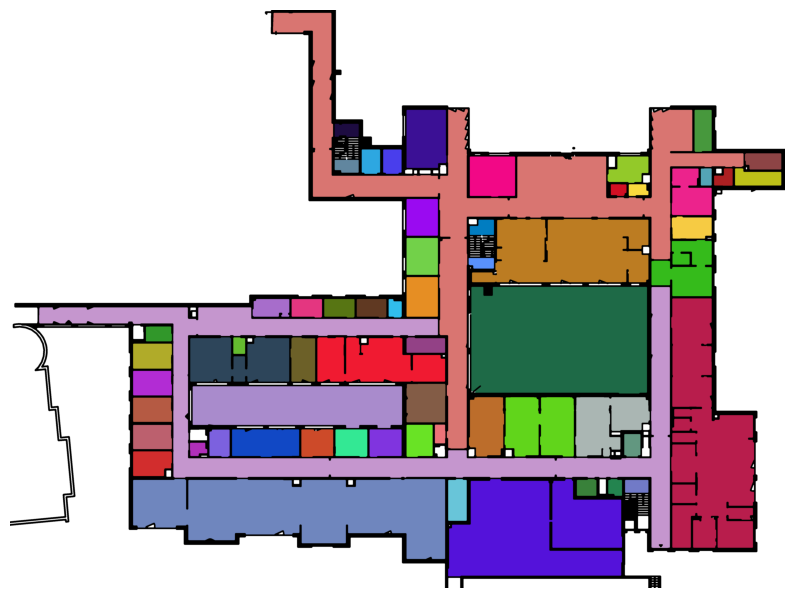
\includegraphics[width=0.48\linewidth]{figures/02.contours_image.png}
    \caption{Example of rooms detections using \texttt{VisionSegmentation}. 
    Left: Binary image generated from vector segments. 
    Right: Colorized visualization of detected rooms. Room without doors are merged in this version.}
    \label{fig:geojson_and_colored}
\end{figure}


\paragraph{Discussion}
This vision model offers a simple yet robust solution for room segmentation on 
vector floor plans. It avoids the complexity of enforcing strict topological 
rules in vector space and instead leverages the flexibility of raster-based computer 
vision techniques. The method is particularly suited to noisy, exports where 
traditional vector-based approaches may struggle.

However, the \texttt{VisionSegmentation} also depends on the explicit representation of physical separations. 
In cases where doors are missing, or open connections are not physically modeled, 
adjacent spaces may be incorrectly merged into a single room.


% =============================================================================
% Fm @Aboul
\subsection{Model 3: \texttt{SAM}, Based on Segment Anything}
To handle the open door issue, we explore another vision-based model 
based on the Segment Anything Model 
(SAM)\cite{kirillov2023segment}. SAM is a foundation model for image and videos segmentation. Developed by 
Meta's FAIR (Fundamental AI Research) lab, SAM represents a significant advancement 
in computer vision, designed to serve as a versatile framework for various 
segmentation tasks. His architecture can be summarized in three parts: a Vision 
transformer image encoder, a prompt encoder, and a modified mask Transformer decoder
 block (see Figure \ref{fig:SAMmodel_diagram}, taken from original paper \cite{kirillov2023segment}).
 Further details and pipeline description 
 can be found in appendix \ref{app:sec:SAMdetails}. 

\paragraph{Discussion}
This model is way more computationally expensive than the two previous ones, 
and requires GPU memory to detect rooms in seconds. It correctly splits
the non-connected rooms and is able to detect rooms without doors.
However, the model is not as precise as the other ones.


% =============================================================================
% Section results
% =============================================================================

\section{Results}
% \textit{Provide convincing plots/tables to support your conclusions.\\
% Justify the metrics you have used to compare methods/assess performance.}

\subsection{Construction of a Metric}
\label{sec:metric}
The classical metric for segmentation tasks is the Intersection over Union (IoU).
But in the specific context of room detection, we define a \textbf{matched IoU
metric} that considers the intersection over union of the detected room with the
ground truth room that matches the more with the detection.
This adaptation is further described in appendix 
\ref{app:sec:IoUdetails}. It computes a score from 0 (no match) to 1 (perfect 
overlapping). 
\subsection{The Results}
Figure \ref{fig:result_segmentation} displays the evaluation of 2 models on a single 
plan. The darker the green the better the score of the individual rooms. This metric 
penalizes our model when it split a merged room from the ground truth despite a 
wall drawn in plan. Furthermore, our models do not detect rooms open to the sides
of the image as a consequence of the application of expert rule.
\begin{figure}[h]
    \centering
    \begin{tabular}{cc}
        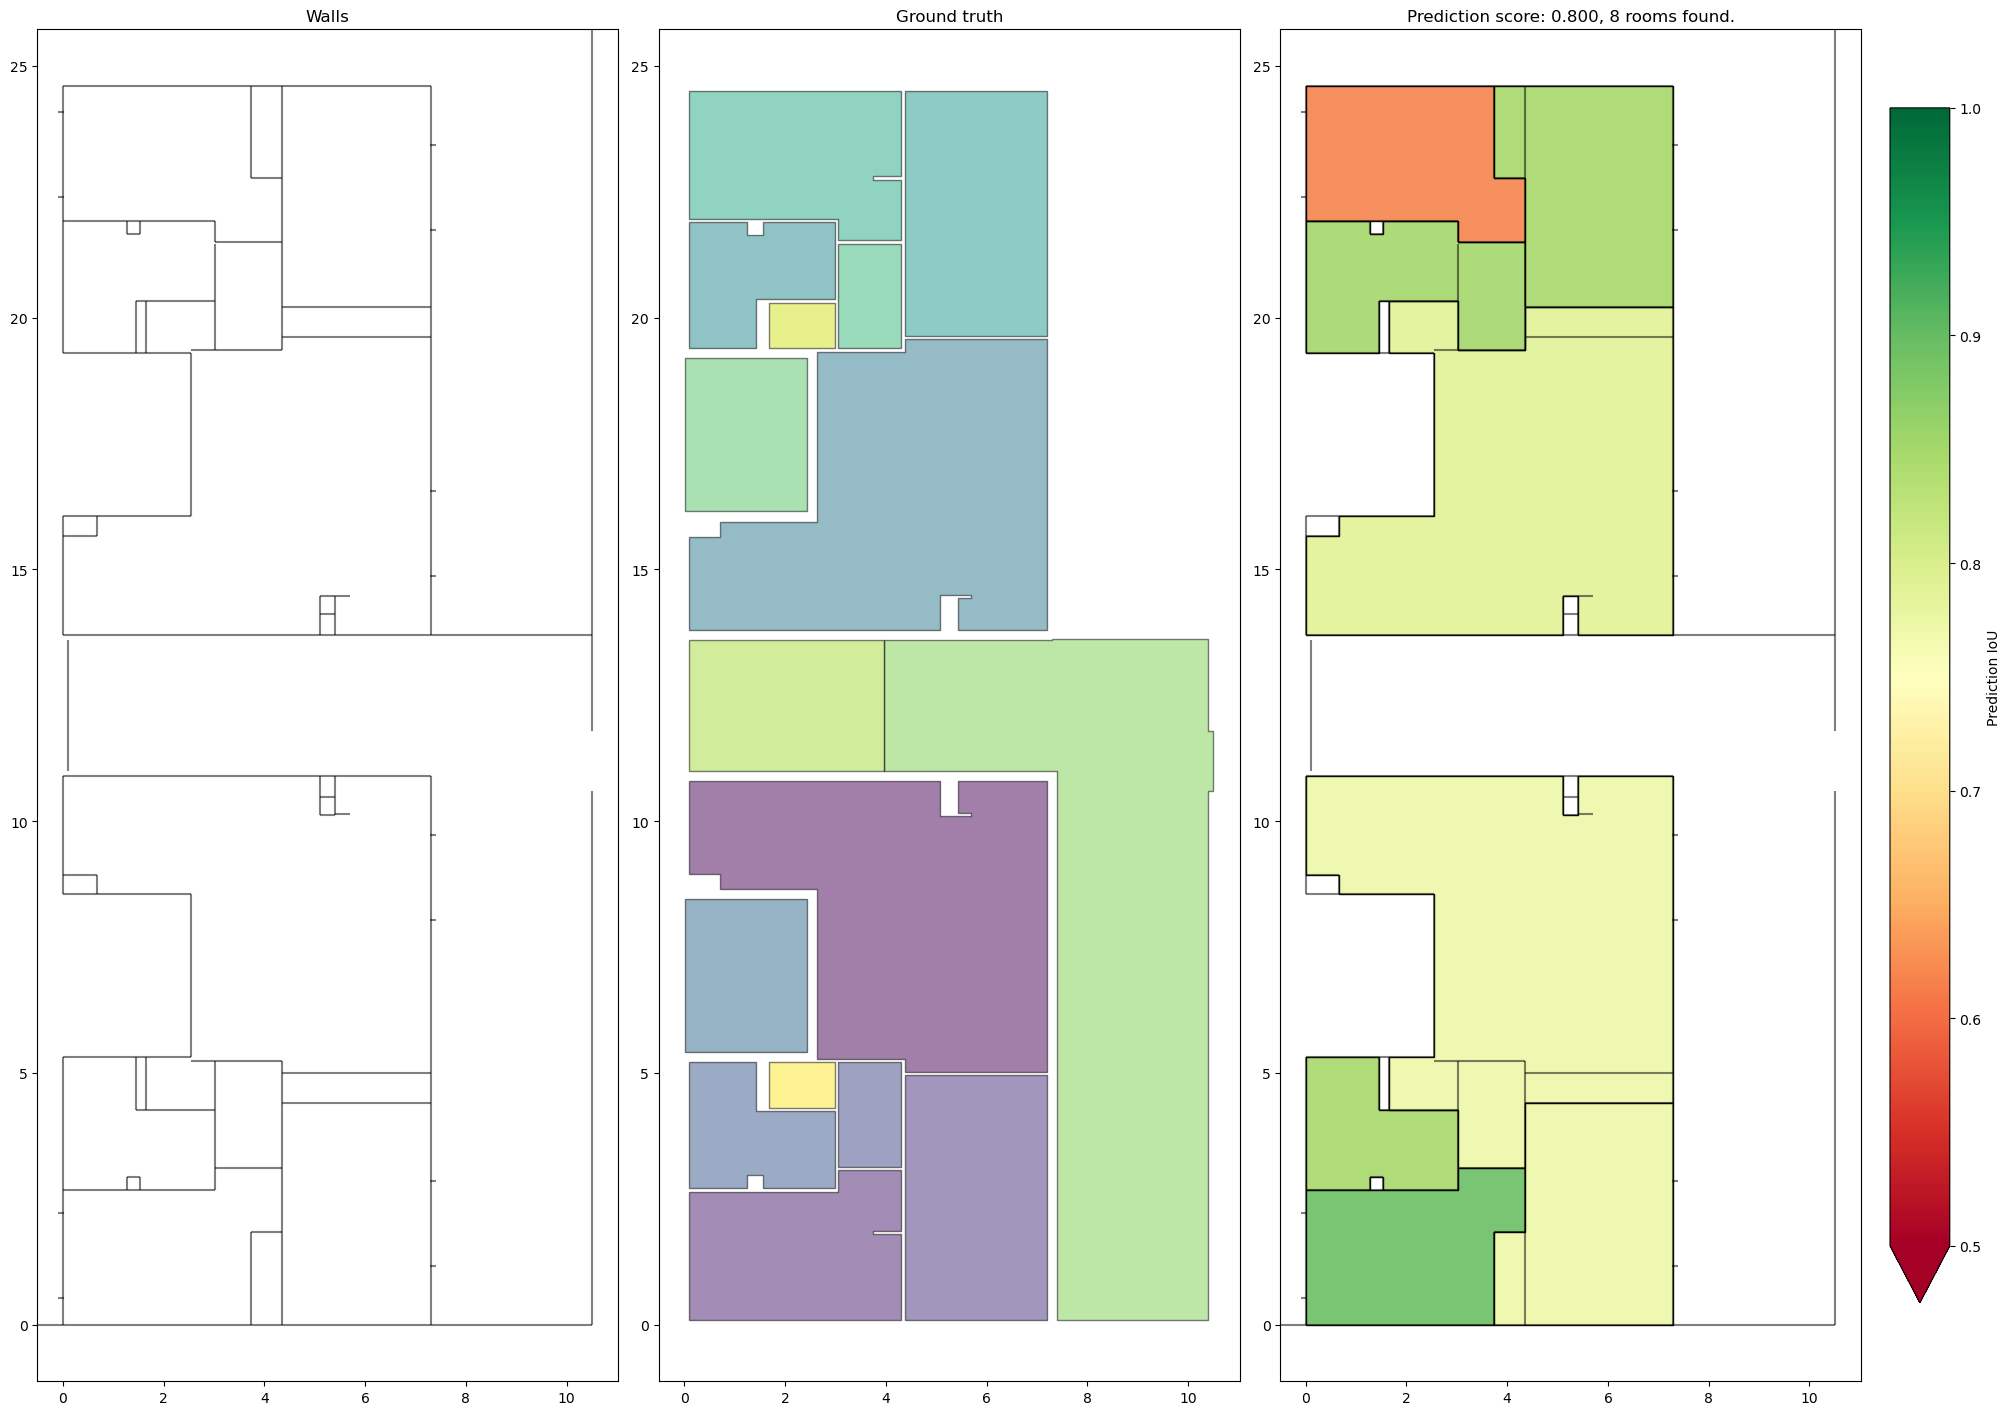
\includegraphics[width=0.45\linewidth]{figures/ScoreSeg.png} &
        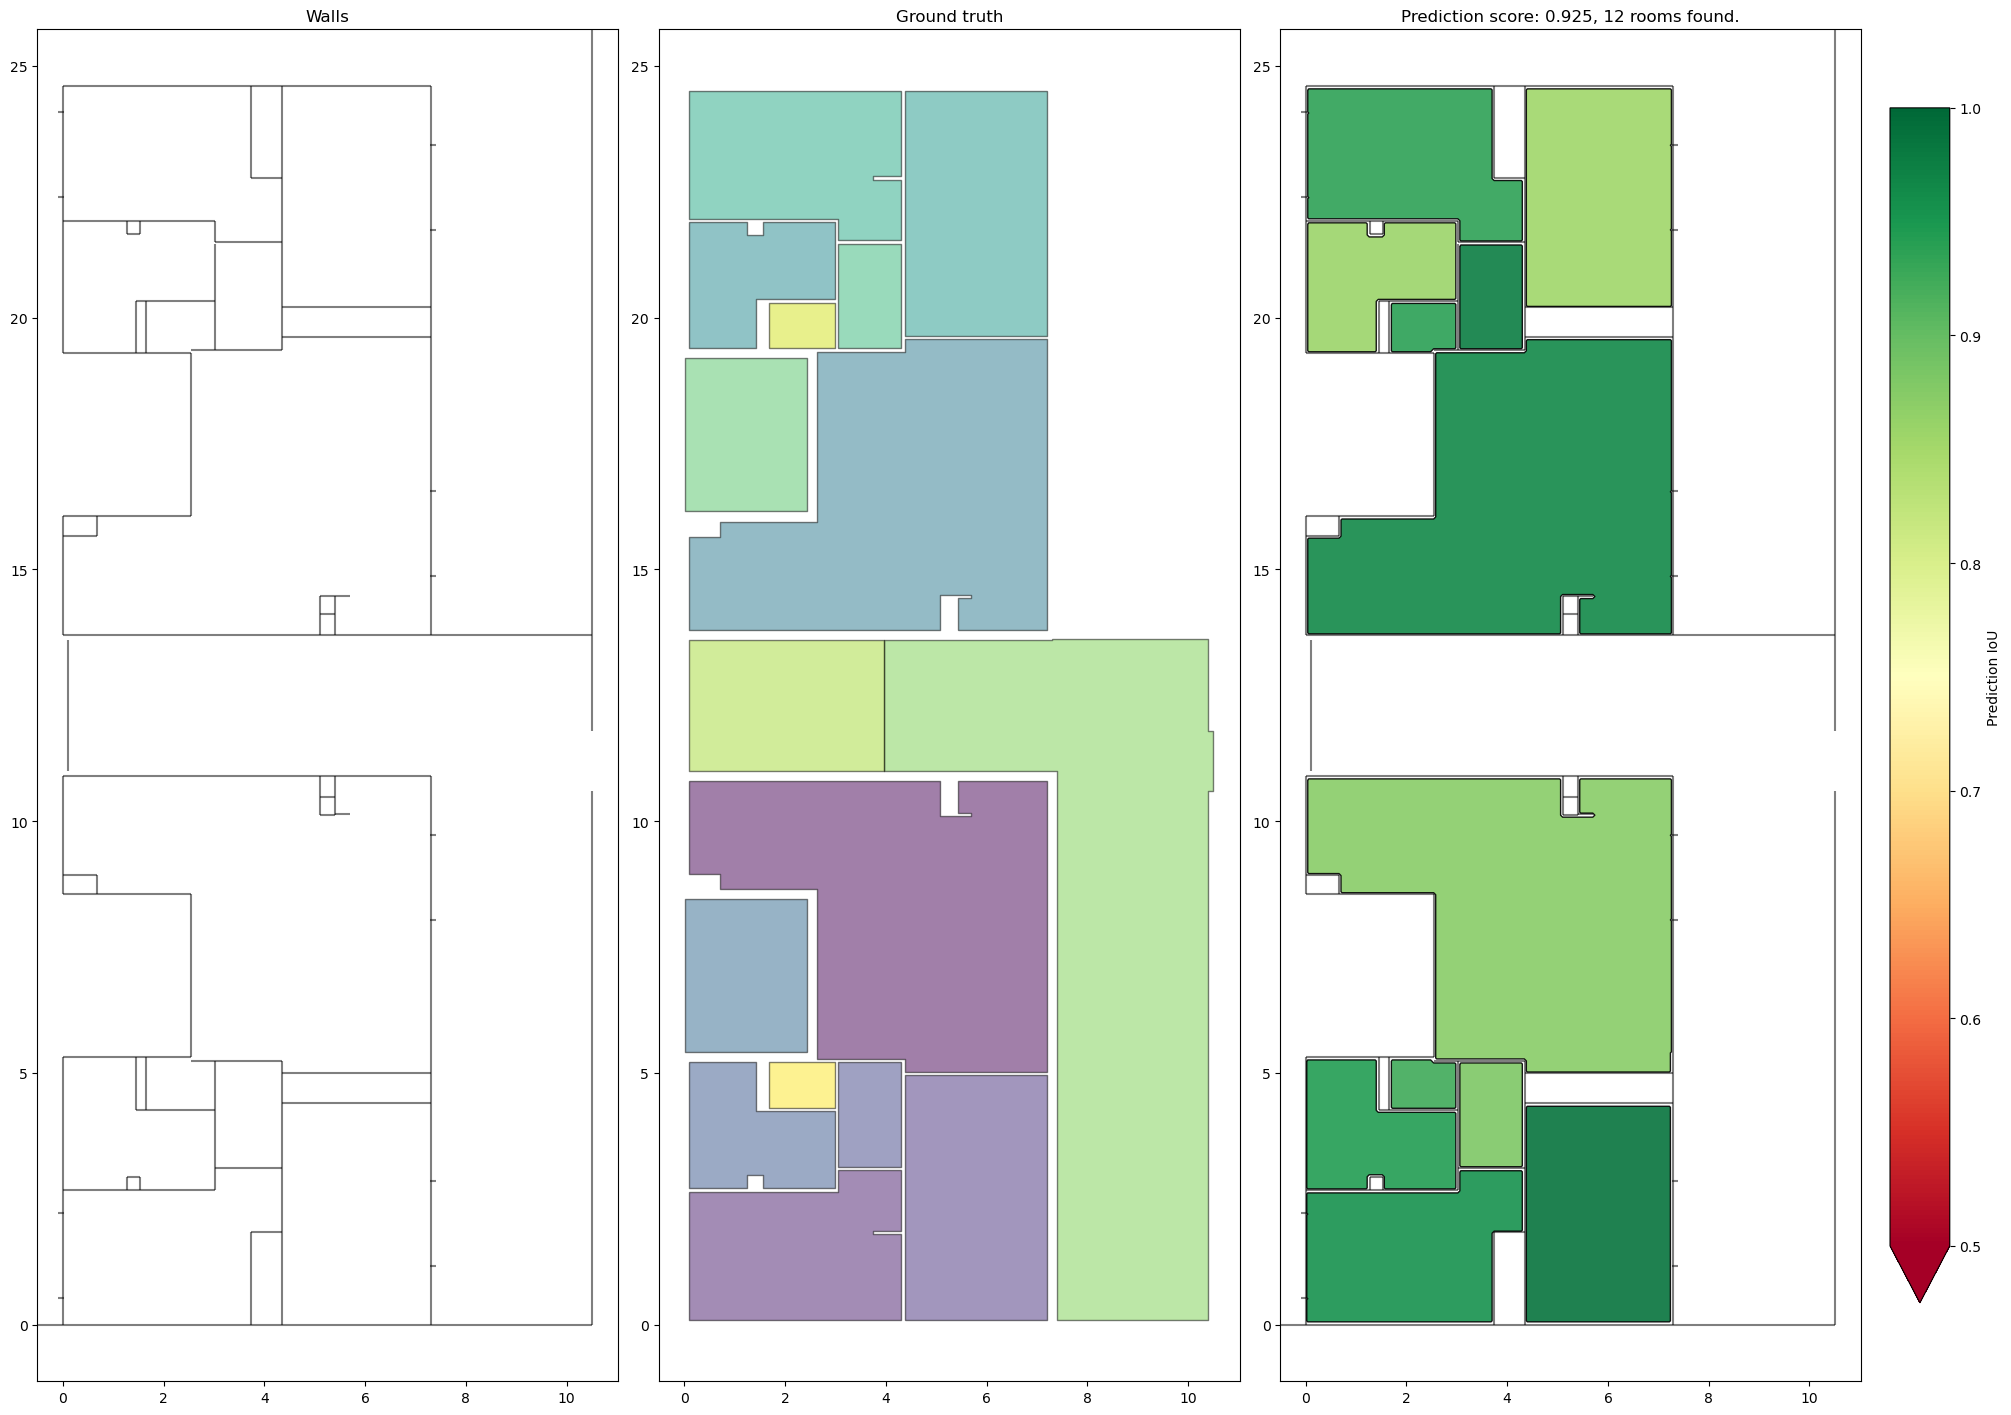
\includegraphics[width=0.45\linewidth]{figures/ScoreCV.png} \\
        
    \end{tabular}
    \caption{Visualization of original walls / predictions / scoring of the two first models 
    on the same plan
    (left: \texttt{SegmentBasedClustering}, right: \texttt{VisionSegmentation}).}
    \label{fig:result_segmentation}
\end{figure}

Additionally, we conducted a comparison of the three models on the second dataset.
The final results are summarized in table \ref{tab:results} and shows a trade-off 
for \texttt{VisionSegmentation}.
\begin{table}[hb!]
    \centering
    \begin{tabular}{|l|c|c|c|}
        \hline
        \textbf{Model} & \textbf{Mean IoU} & \textbf{Mean Matched IoU} & \textbf{Time} \\
        \hline
        \texttt{SegmentBasedClustering} & 0.04 & 0.76 & 6.8s \\
        \texttt{VisionSegmentation} & 0.09 & 0.86 & 4.6s \\
        \texttt{SegmentAnythingModel} & ? & ? & ?s \\
        \hline
    \end{tabular}
    \caption{Comparison of the three models on the second dataset.}
    \label{tab:results}
\end{table}

Our models have variant performances overs the different plans. The two
first models are very sensitive to the open doors but are more precise and 
faster than the last one. The last one is more robust but less precise and
more computationally expensive.

\section{Conclusion}
% \textit{Summarize and discuss the main findings. What are the limitations?\\
% Are the experiments conclusive? With more time, what else would you have tried?}
\paragraph{Main findings}
This project is amazing in a sense that it is very easy to understand but very hard
to solve when digging into it. We really enjoyed the freedom given by Vinci/Diane
to explore different paths and to come up with different solutions. We have
also benefited from their expertise to guide us in the right direction and avoid
death traps. 
Our team is pretty proud to have managed to produce three models that are actually able to
detect the contours of the rooms in the floor plans. They are not perfect, but
they are working and respect the requested workflow.

\paragraph{Limitations}
The models are sensitive to the representation of the plans. Furthermore, we 
were not able to find an efficient algorithm to close the doors and other corridors.
An other improvement would be to discriminate wide walls that are sometimes 
identified as rooms.

\paragraph{Organization within the team}
%\textit{How did you share the work among yourselves? (short paragraph, 1/2 page max)}
The project initially started in the office of Vinci/Diane for a brainstorming session.
Since then, we have been working remotely in a smooth way, meeting with 
Vinci/Diane at the beginning of each Thursday afternoon. We were using a shared 
git repository to share our code and results\footnote{Private: https://github.com/waddason/CapstoneContour}.

After a first quick diverging phase where every one has 
tried different methods and dug into the data,  we have split in teams of two 
to focus on two paths described in \cref{sec:methods}. Tristan took care of the global information management process and organized the
relations with Vinci.
\begin{itemize}
    \item Tristan handled the initial data cleaning, then worked with Maha who 
    expertly created the geometric process and the segment preprocessing and clustering.
    \item Abdoul explored first the computer vision path and Fabien made the 
    breakthrough in the results with the image segmentation.
\end{itemize}


% =============================================================================
% Bibliography (automatic)
% =============================================================================

% Automatic bibliography form references.bib
\bibliographystyle{plain}
\bibliography{references}

% =============================================================================
% Appendix
% =============================================================================

\appendix

\newpage
%The appendix does not count towards the 5-page limit. 
% =============================================================================

\section{Additional details on the geometric preprocessing}
\label{app:sec:geomdetails}
\paragraph{Preprocessing Results}

This preprocessing step is particularly effective for large datasets with high 
redundancy, as it reduces computation complexity while maintaining architectural 
integrity. But it can be problematic when applied to smaller input datasets like 
in our third example. So it should be used with caution, as excessive modification 
of small datasets can worsen distortions, as seen with 520 segments where a 0.443m 
displacement occurred. As a consequence, the preprocessing step is an option when
using our models.

\begin{figure}[h]
    \centering
    \begin{tabular}{ccc}
        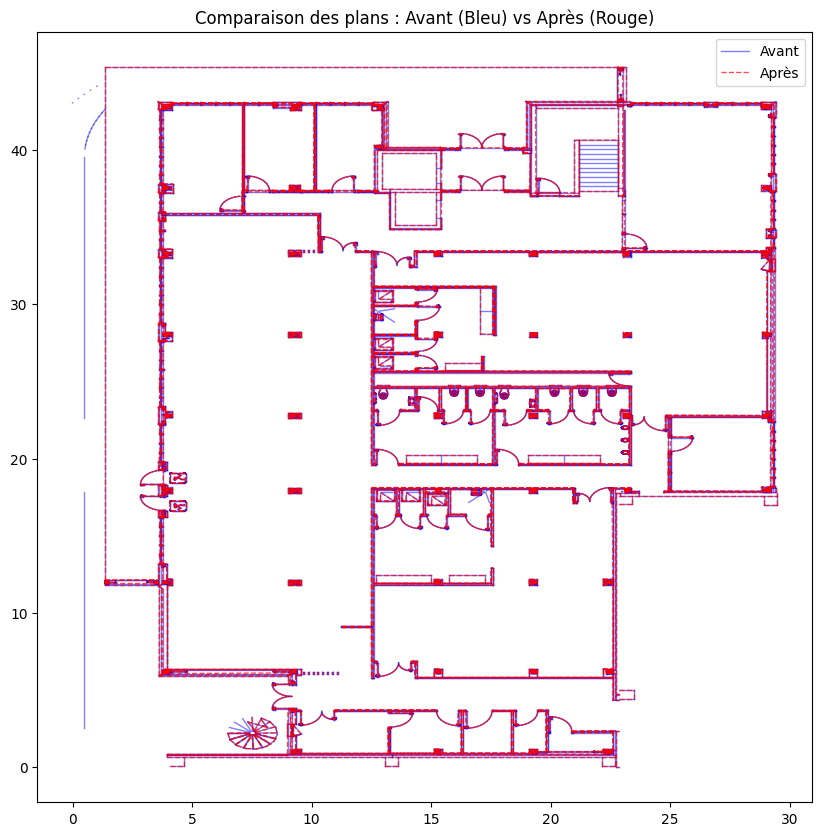
\includegraphics[width=0.32\linewidth]{figures/avant_apres_pretraitement2.png}
        &
        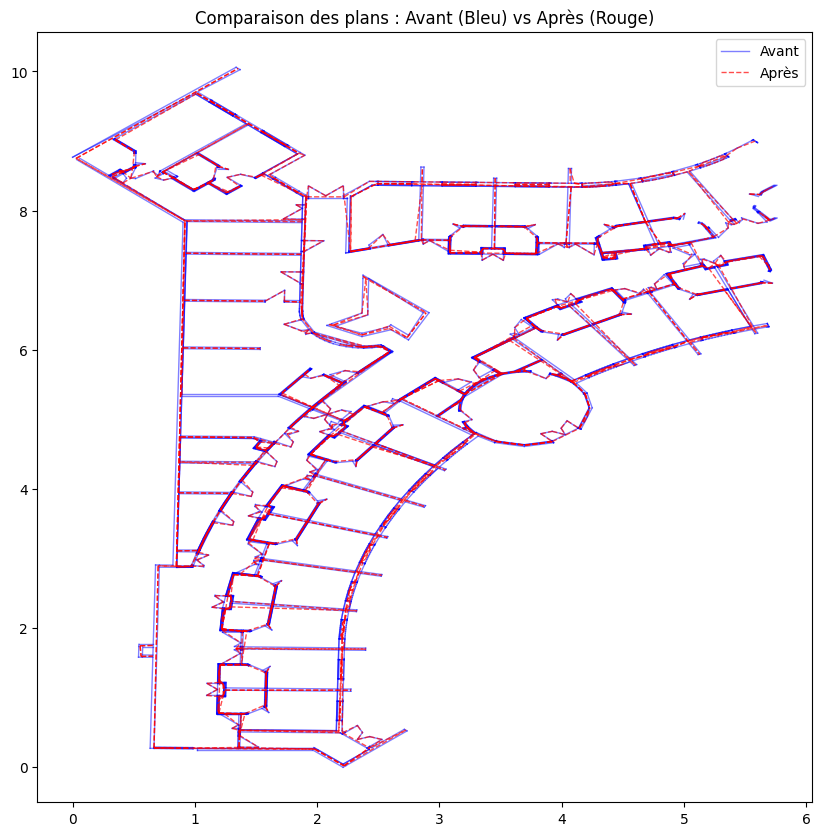
\includegraphics[width=0.32\linewidth]{figures/avant_apres_pretraitement7.png}
        &
        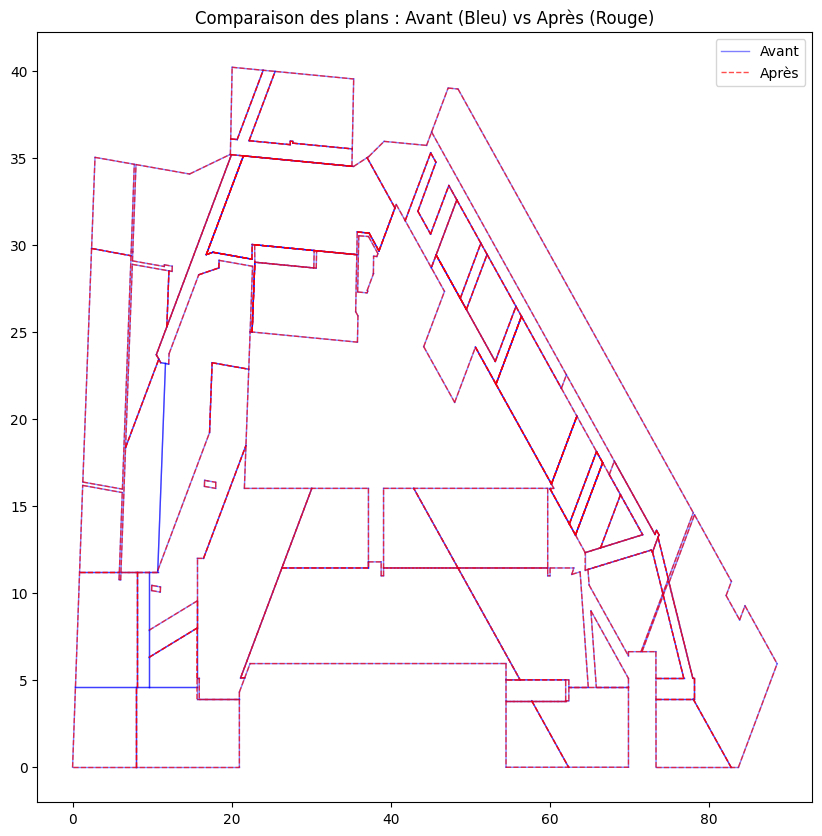
\includegraphics[width=0.32\linewidth]{figures/avant_apres_pretraitement3.png}
        \\
        Case1: output2 & Case2: output7 & Case3: output3 
    \end{tabular}

    \caption{Comparison of floor plans before (Blue) and after (Red) preprocessing 
    for 3 different floor plans. The near absence of blue segments proves that
    we have removed a lot of noise.}
    \label{fig:geojson_comparison}
\end{figure}
The following tables summarize the impact of the geometric preprocessing on the
segment count and the average displacement after preprocessing. We used three 
different floor plans that spans along the range of complexity of the dataset.

The drop in segment count is significant, with a reduction of over 70\% in most cases, 
reducing computational cost of the ulterior tasks. See table \ref{tab:segment_count} for details.

\begin{table}[htb!]
    \centering
    \begin{tabular}{|l|rrc|}
        \hline
        \textbf{Test Case} & \textbf{Nb segments before} & \textbf{Nb segments after} & \textbf{Reduction \%} \\
        \hline

        Case 1 & 22,425 & 6,417 & 71.38\% \\
        Case 2 & 6,013 & 1,648 & 72.59\% \\
        Case 3 & 520 & 330 & 36.54\% \\
        \hline
    \end{tabular}
    \caption{Impact of geometric preprocessing on segment count.}
    \label{tab:segment_count}
\end{table}

This drop in segment count comes with a light cost in the accuracy of the representation.
On most cases, the segments are moved of about 2 cm, which is acceptable for the
purpose of the project. See table \ref{tab:avg_displacement} for details.

\begin{table}[htb!]
    \centering
    \begin{tabular}{|l|c|}
        \hline

        \textbf{Test Case} & \textbf{Avg. Displacement} \\
        \hline
        Case 1 & 0.02 \\
        Case 2 & 0.025 \\
        Case 3 & 0.443 \\
        \hline

    \end{tabular}
    \caption{Average displacement after preprocessing.}
    \label{tab:avg_displacement}
\end{table}

In our code, this preprocessing is done with the method 
\texttt{preprocess\_segments\\.complete\_preprocessing(segments, angle\_tol=0.1, distance\_tol=0.3, snap\_tol=0.05)\\ -> cleaned\_segments}. 
    Where \texttt{angle\_tol} is the maximum angle between two segments to be considered collinear,
    \texttt{distance\_tol} is the maximum distance between two segments to be considered collinear,
    and \texttt{snap\_tol} is the maximum distance between two endpoints to be snapped together.

% =============================================================================

\section{Additional details about SegmentBasedClustering model}
\label{app:sec:SBCdetails}
\paragraph{Pipeline Description} The pipeline follows a sequence of geometric operations performed using the 
\texttt{Shapely} computational geometry library.

\begin{enumerate}
    \item  Extracting relevant \textbf{wall segments} from GeoJSON data.
    \item Identifying \textbf{closed loops} using geometric operations.
    \item Retaining valid rooms based on predefined \textbf{area constraints}, 
    considering only polygons between $1 \text{ m}^2$ and $1000 \text{ m}^2$ (hyperparameters).
    \item Identifying which rooms share \textbf{common boundaries} by doing adjacency 
    analysis to facilitate merging and spatial organization.
    \item \textbf{Combining and merges small rooms} (under $5 \text{ m}^2$) with their 
    largest adjacent neighbor.
\end{enumerate}

% =============================================================================
\section{Additional Details about \texttt{VisionSegmentation} Model}
\label{app:sec:CVdetails}
\paragraph{Pipeline Description}
The method is structured in the following key steps:

\begin{enumerate}
    \item \textbf{Vector Preprocessing.}  %% TODO like in previous session
    Raw GeoJSON data often includes heterogeneous geometries (Polygons, 
    MultiPolygons, LineStrings), many of which are noisy or incomplete. 
    We filter the data to retain only the linear primitives representing walls. 
    The geometries are rescaled and recentered to ensure consistent metric 
    resolution before conversion. This corresponds to the steps (i) and (ii)
    described in the geometric preprocessing in section \ref{sec:geometric_preprocess}.

    \item \textbf{Binary Image Generation.} 
    The preprocessed segments are rasterized into binary black-and-white images,
    where each segment is drawn with a configurable thickness (default: 3 pixels).
    A DPI value of 50 (pixels per meter) ensures sufficient spatial resolution. 
    To improve the connectivity of wall segments, we apply Gaussian dilation, 
    which smooths the edges and \emph{ensures continuity} even in curved or 
    oblique wall segments. Result is shown on figure \ref{fig:geojson_and_colored} left.

    \item \textbf{Morphological Processing and Contour Detection.} 
    A morphological closing operation (\texttt{cv2.morphologyEx} with \texttt{MORPH\_CLOSE} operation) fills
     small gaps between wall segments. Contours are then extracted with 
     \texttt{cv2.findContours} using the \texttt{RETR\_CCOMP} mode, producing a 
     hierarchical tree structure that allows holes (e.g., internal courtyards 
     or voids) to be identified and processed correctly.

    \item \textbf{Wall Filtering and Room Selection.} 
    To discriminate between rooms and walls, we apply geometric criteria. 
    Only contours with a surface area greater than 1 m² (2500 pixels at 50 DPI) 
    and an average thickness (surface-to-perimeter ratio) exceeding 0.4 meters 
    are retained. Best parameters displayed in table \ref{tab:CV_model_checkpoint}
    have been found using the validation dataset. 

    Additionally, the longest contour—typically representing the 
    building envelope—is discarded. The detected rooms are shown on figure 
    \ref{fig:geojson_and_colored} right.

    \item \textbf{Polygon Conversion and GeoJSON Export.} 
    The valid contours are converted back into metric coordinates using 
    transformation parameters from the rasterization step. Polygons are enriched 
    with properties such as area (m²) and a unique room identifier. Final outputs 
    are exported in GeoJSON format to be loaded back into CAD software.
    
\end{enumerate}

\paragraph{Hyperparameters tuning}
An extensive hyperparameter search was conducted to optimize the model's
performance. The best parameters are summarized in table \ref{tab:CV_model_checkpoint}.

Numerous tests were conducted using the validation test as a benchmark and using
the matched IoU score to select the best parameters. Example of experiments during the 
early stage of the project are shown in figure \ref{fig:hyperparameters_tuning}.
The DPI value of 50 pixels was kept, but Fabien managed to optimize the code to 
reduce the thickness from 7 to 3 pixels only. This produced contours closer to the 
actual walls.

\begin{figure}[htb!]
    \centering
    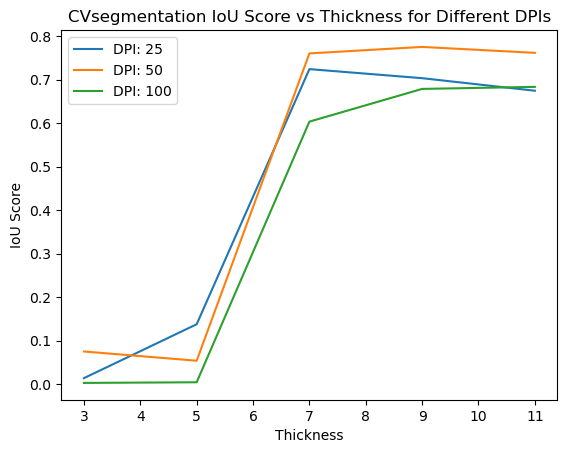
\includegraphics[width=0.5\linewidth]{figures/CVsegmentation_score.png}
    \caption{Example of hyperparameters tuning during the
    early stage of the project.}
    \label{fig:hyperparameters_tuning}
\end{figure}

Ultimately, Fabien developed a dynamic interface to visually check the effects 
of the parameters on the segmentation. This tool was used to fine-tune the
parameters and to define their default values. An illustration of the interface 
is depicted bellow in figure \ref{fig:interface}.

\begin{figure}[hp!]
    \centering
    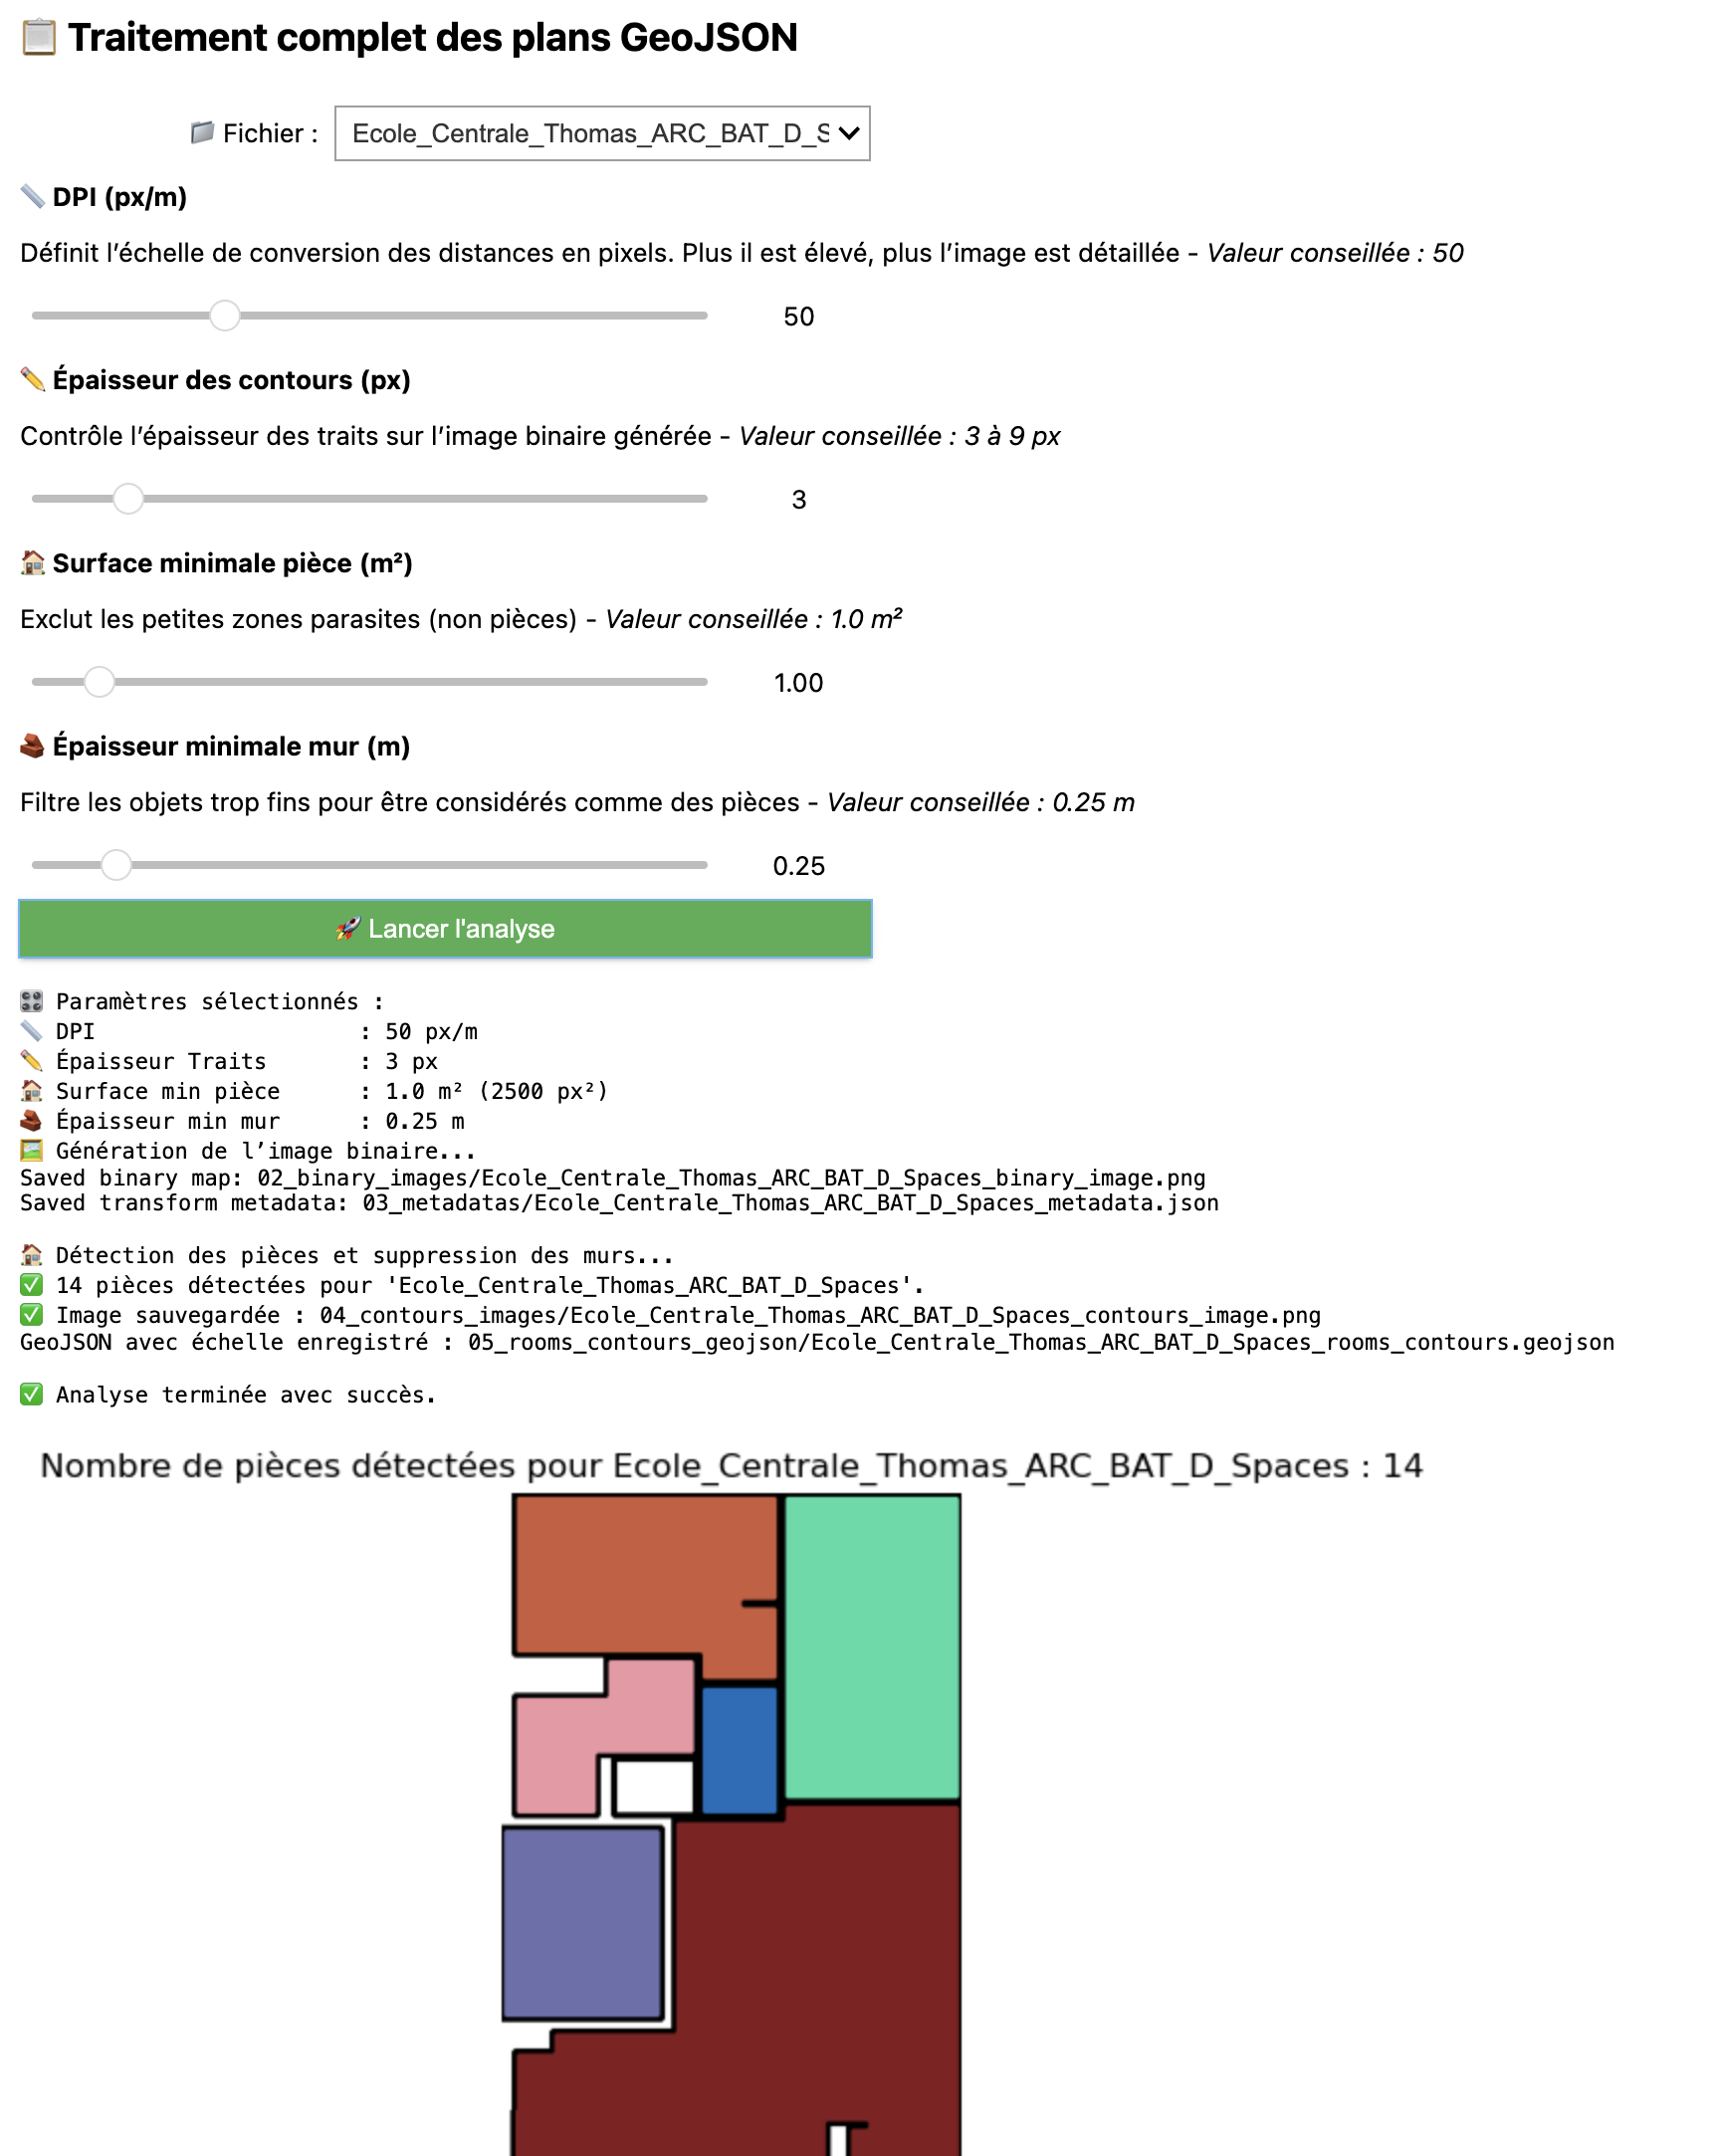
\includegraphics[width=1\linewidth]{figures/interface.png}
    \caption{Dynamic interface to fine-tune the parameters of the \texttt{VisionSegmentation} model,
    launched inside a Jupyter notebook.}
    \label{fig:interface}
\end{figure} 


\begin{table}[htb!]
    \centering
    \begin{tabular}{|l|l|}
        \hline
        \textbf{DPI} & 50 pixels per meter (1 pixel $\approx$ 2 cm) \\ \hline
        \textbf{Wall thickness} & 3 pixels (default) \\ \hline
        \textbf{Minimum room area} & 1 m² \\ \hline
        \textbf{Minimum average thickness} & 0.4 m \\ \hline
        \textbf{Dilation method} & Gaussian \\ \hline
    \end{tabular}
    \caption{Best \texttt{VisionSegmentation} Model Parameters}
    \label{tab:CV_model_checkpoint}
\end{table}

% =============================================================================

\section{Additional Details about \texttt{SAM} Model}
\label{app:sec:SAMdetails}

\paragraph{Pipeline Description} 
We first produce a high-quality image using the 
two first steps of the \texttt{VisionSegmentation} pipeline presented earlier.
Then, we use SAM to infer masks on 
the image as segmentation of all the rooms. This step require access to GPU.
Finally, the contours of the masks 
are extracted, and after rescaling the contour coordinates, we generate the 
corresponding GeoJSON file. The SAM checkpoint used is described in table
\ref{tab:SAM_model_checkpoint}.

\begin{table}[htb!]
    \centering
    \begin{tabular}{|l|l|}
        \hline
        \textbf{Checkpoint} & \texttt{sam\_vit\_h\_4b8939.pth} \\ \hline
        \textbf{Backbone Size} & Huge (ViT-H) \\ \hline
        \textbf{Model Parameters} & 636 million \\ \hline
        \textbf{File Size} & 2.4 GB \\ \hline
        \textbf{GPU Memory Requirement} & At least 8 GB \\ \hline
        \textbf{Use Case} & Tasks requiring high-quality segmentation \\ \hline
    \end{tabular}
    \caption{\texttt{SAM} Model Checkpoint Information}
    \label{tab:SAM_model_checkpoint}
\end{table}


\begin{figure}[htb!]
    \centering
    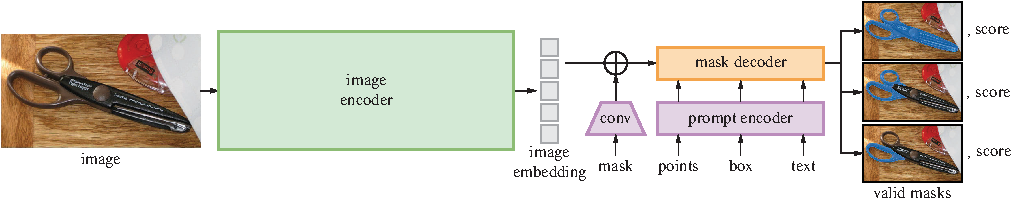
\includegraphics[width=0.9\linewidth]{figures/SAM_model_diagram.pdf}
    \caption{Segment Anything Model (SAM) overview}
    \label{fig:SAMmodel_diagram}
\end{figure}


% =============================================================================

\section{Additional Details about the Intersection over Union Metric}
\label{app:sec:IoUdetails}
During their extensive review of the literature, the Chillian team of
Pizarro et al.\cite{PIZARRO2022104348}, 
found several possible
metrics to evaluate the performance of the models. 
Typically, segmentation results were evaluated in terms
of the intersection over union (IoU), pixel/class accuracy, and
the Jaccard Index (JI) proposed by de Las Heras et al.. By contrast, works that 
detected objects (e.g., walls, doors, windows) used
the mean average precision (mAP), the recall \& precision, the match
score (MS), detection rate (DR), and recognition accuracy (RA),
or considered a confusion matrix.
Hence, we decide to focus on the IoU metric.

\subsection{IoU for Object Detection}
\paragraph{Definition} The Intersection over Union (IoU) metric is a standard
measure of the accuracy of a segmentation model. It is defined as the ratio of
the area of intersection to the area of union of the Ground Truth (GT) and the 
segmentation mask (S). The mathematical formula is given below, and an illustration
is provided in figure \ref{fig:iou_segmentation}.

\begin{itemize}
    \item True Positive: The area of intersection between Ground Truth (GT) and segmentation mask (S). Mathematically, this is logical AND operation of GT and S i.e.
    $TP = GT.S$,
    \item False Positive: The predicted area outside the Ground Truth. This is the logical OR of GT and segmentation minus GT.
    $FP=(GT+S) - GT$,
    \item False Negative: Number of pixels in the Ground Truth area that the model failed to predict. This is the logical OR of GT and segmentation minus S
    $FN=(GT+S) -S$,
    \item Final IoU: The ratio of the area of intersection to the area of union of GT and S. Mathematically,
    $IoU = \frac{TP}{TP+FP+FN}$
\end{itemize}

\begin{figure}[hb!]
    \centering
    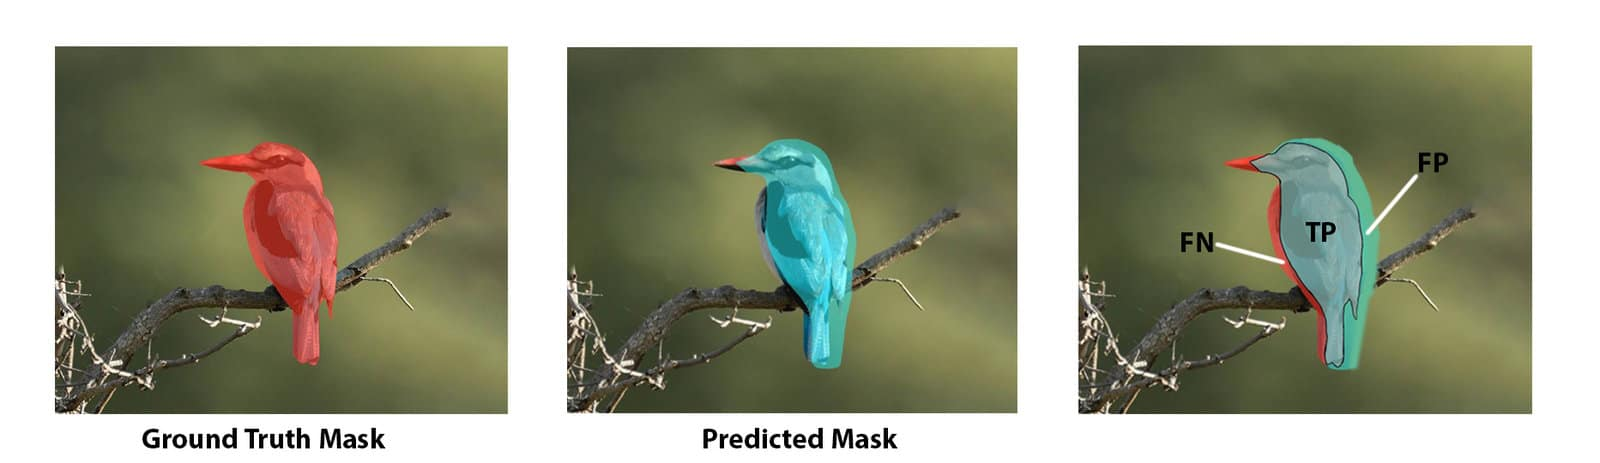
\includegraphics[width=0.5\textwidth]{figures/5-segmentation-iou.jpg}
    \caption{IoU is the ratio of the intersected area to the combined area of
     prediction and ground truth masks. 
     (source: \href{https://learnopencv.com/intersection-over-union-iou-in-object-detection-and-segmentation/}
        {learnopencv.com})}
    \label{fig:iou_segmentation}
\end{figure}

In our code \texttt{utils.metric.intersection\_over\_union(gt, pred) -> float},
compute the score using the ratio of the calculated areas thanks to the powerful
\texttt{shapely} library that provides \texttt{intersection} and \texttt{union} 
methods for polygons.

\subsection{Matched IoU for Room Detection}
\paragraph{Definition} In the context of room detection, we define a \textbf{matched IoU
metric} that considers the intersection over union of the detected room with the
ground truth room that matches the most. 

Initially, the metric is computed as the average IoU over all detected rooms.
Then an optimization algorithm is used to match the detected rooms with the ground truth rooms
to maximize the average IoU. Specifically, we used the Hungarian algorithm from 
Harold Kunhn to solve the
assignment problem, using the \texttt{scipy.optimize.linear\_sum\_assignment} function.
The final metric is the average IoU of the matched rooms.
Despite its complexity, this metric is more informative than the simple IoU metric 
and is more adapted to score our models as the results are closer to 1 (the 
optimal score) than when averaging over all rooms.

\paragraph{Possible extentions}
We choose not to penalize the non-detected rooms, because we 
did not have to train models from scratch. Ultimately, we also define a Jaccard 
loss in the purpose of training future models. But it is not used it in the current project.

% =============================================================================

\section{Additional Segmentation Results}

The figure \ref{fig:segmentation_results} below displays the segmentation results of the three models on random
floor plans. The first line shows the results of the \texttt{SegmentBasedClustering} model,
the second line shows the results of the \texttt{VisionSegmentation} model, and the third line
shows the results of the \texttt{SegmentAnythingModel} model, each with a 
distinctive color map.

The left column shows the prediction on the same plan for comparative purpose. 
On this simple well drawn example, all models correctly detects the rooms and
corridors. 
We note that the \texttt{VisionSegmentation} model get the best results on complex plans (center).
\begin{figure}[hp]
    \centering
    \begin{tabular}{ccc}
        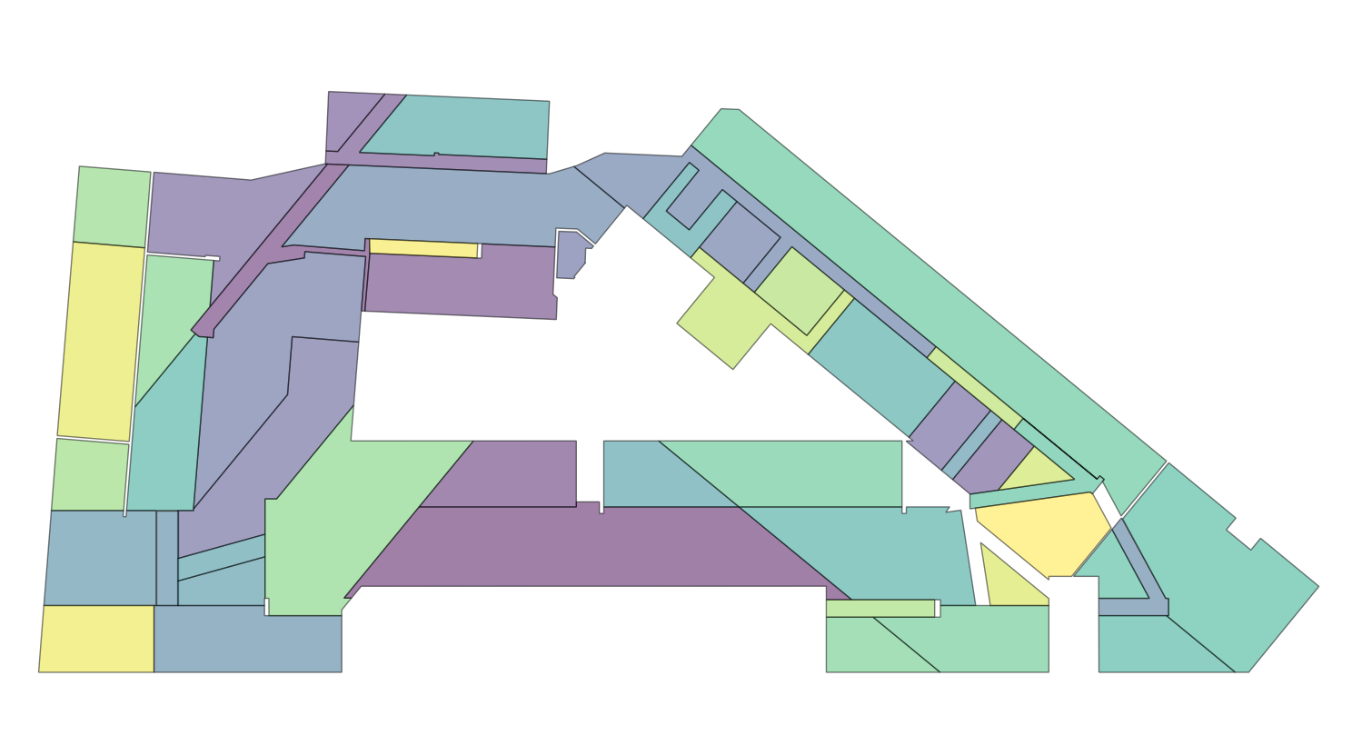
\includegraphics[width=0.3\linewidth]{figures/SBC_pred-4.png} &
        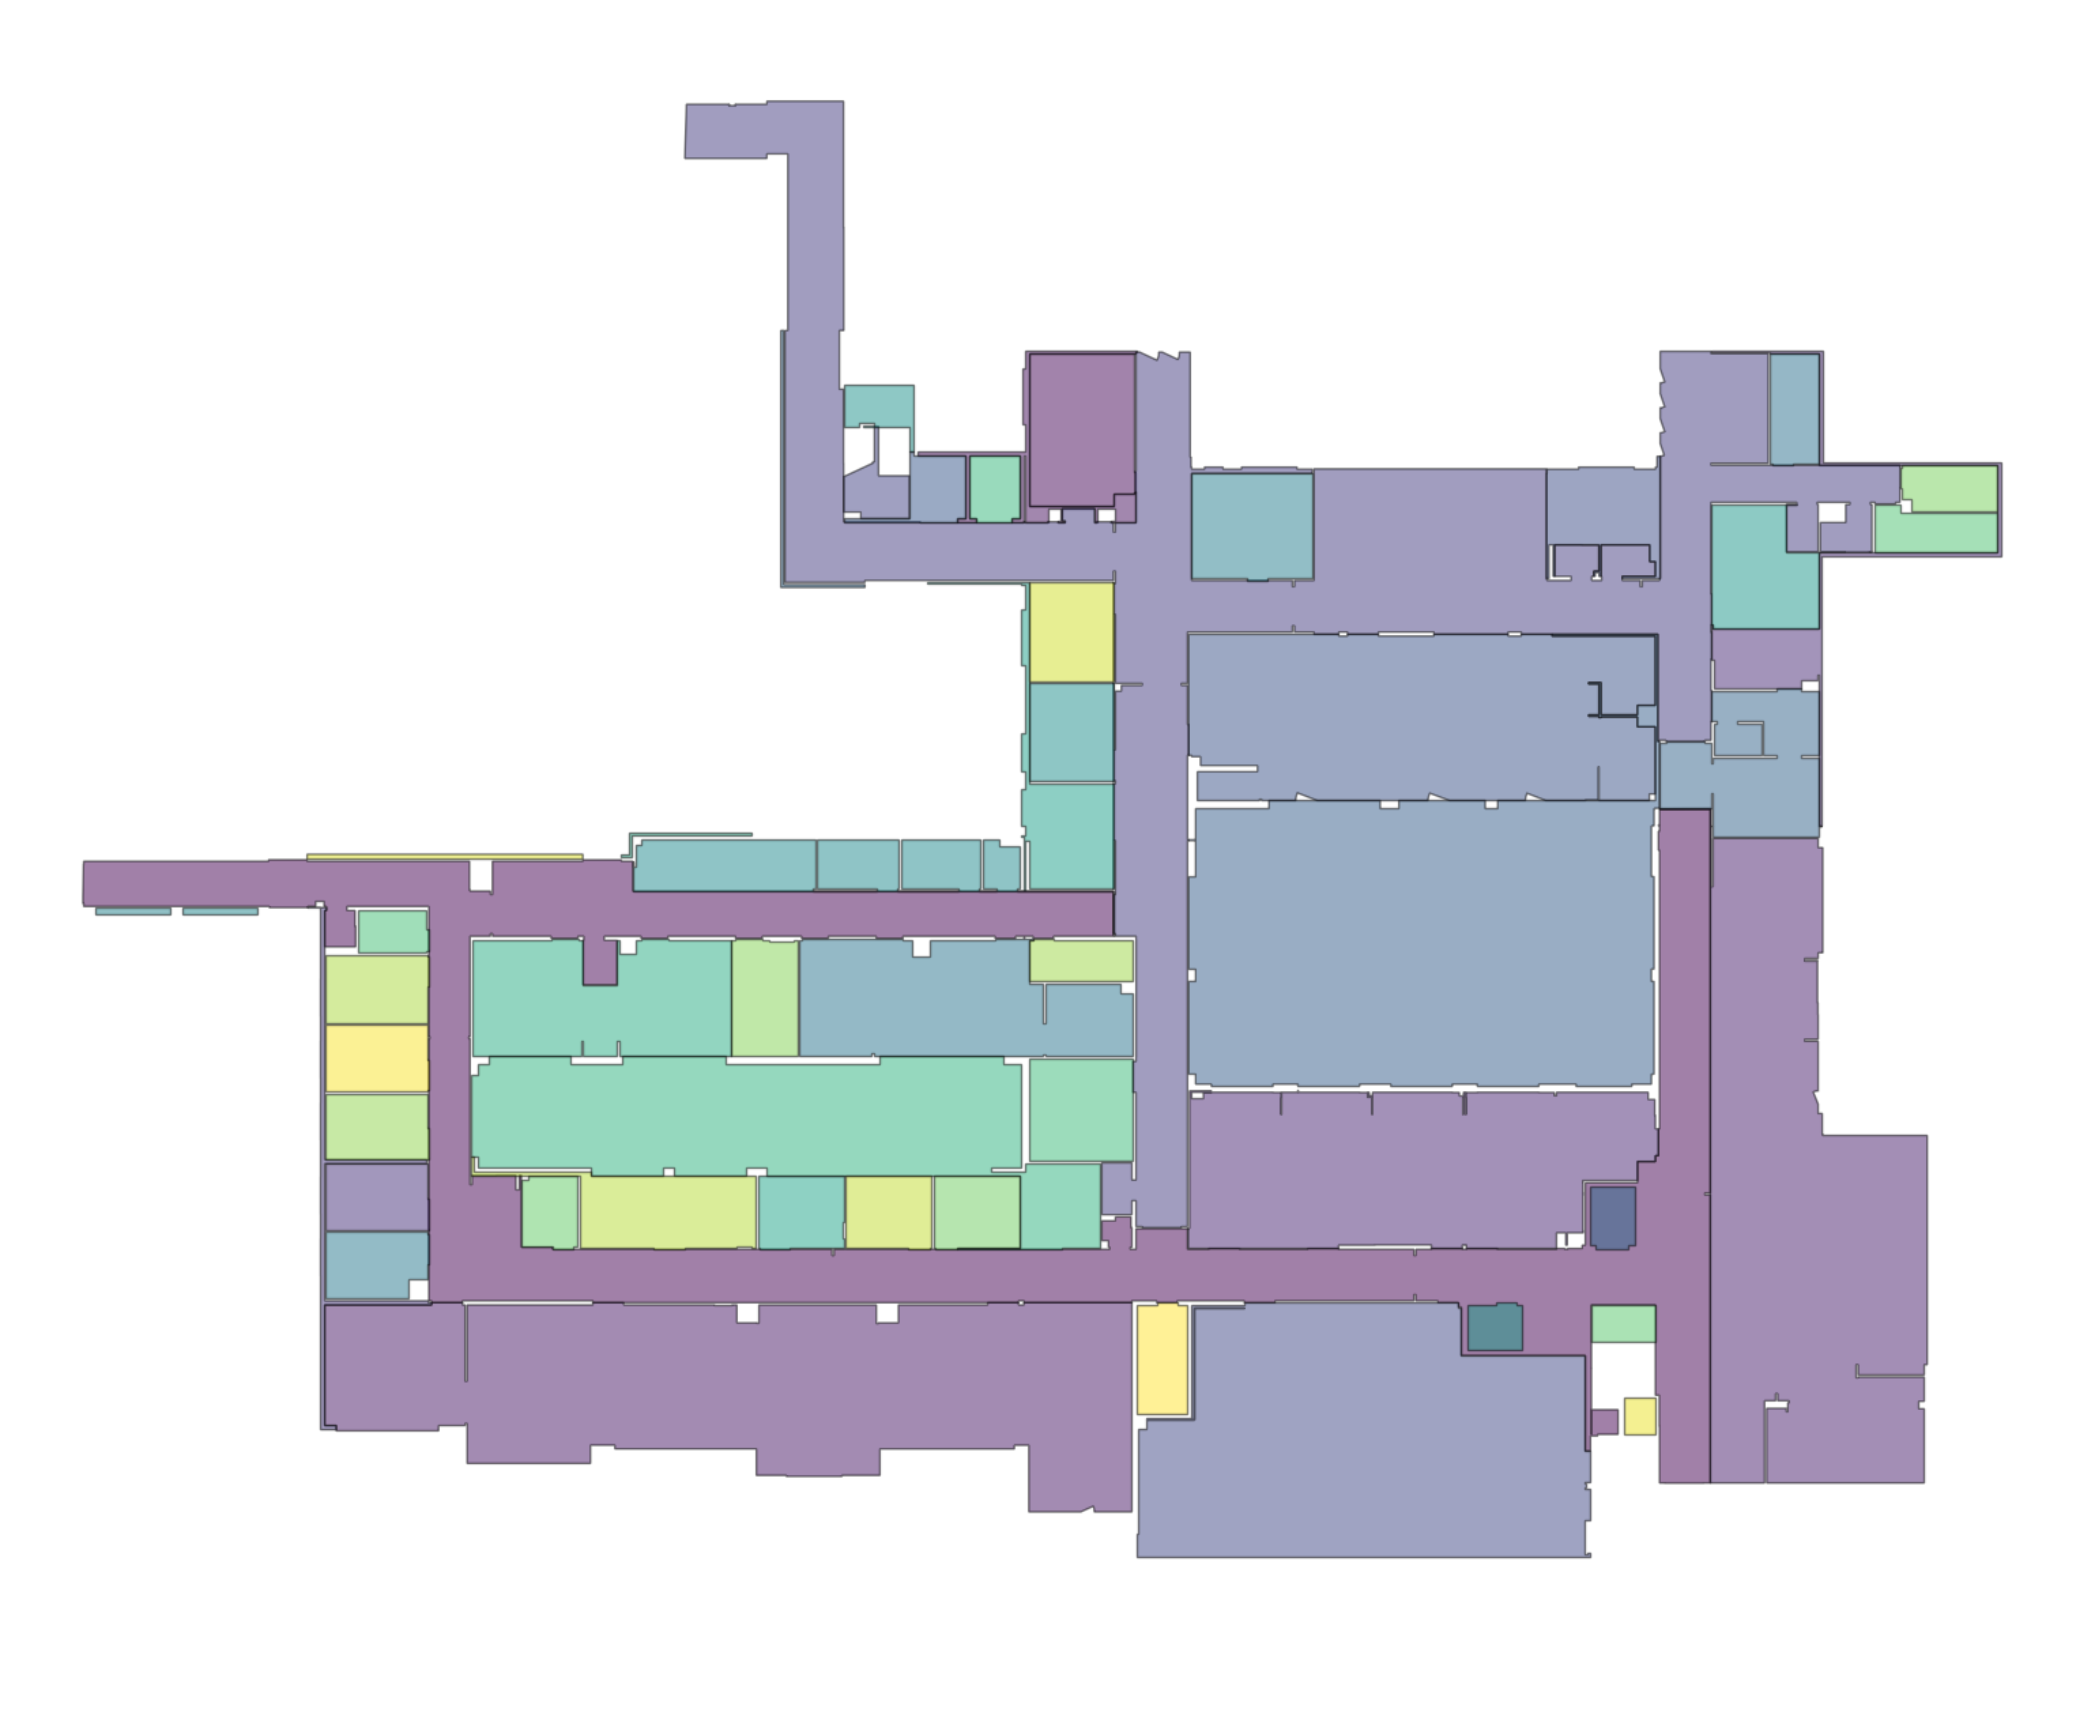
\includegraphics[width=0.3\linewidth]{figures/SBC_pred-3.png} &
        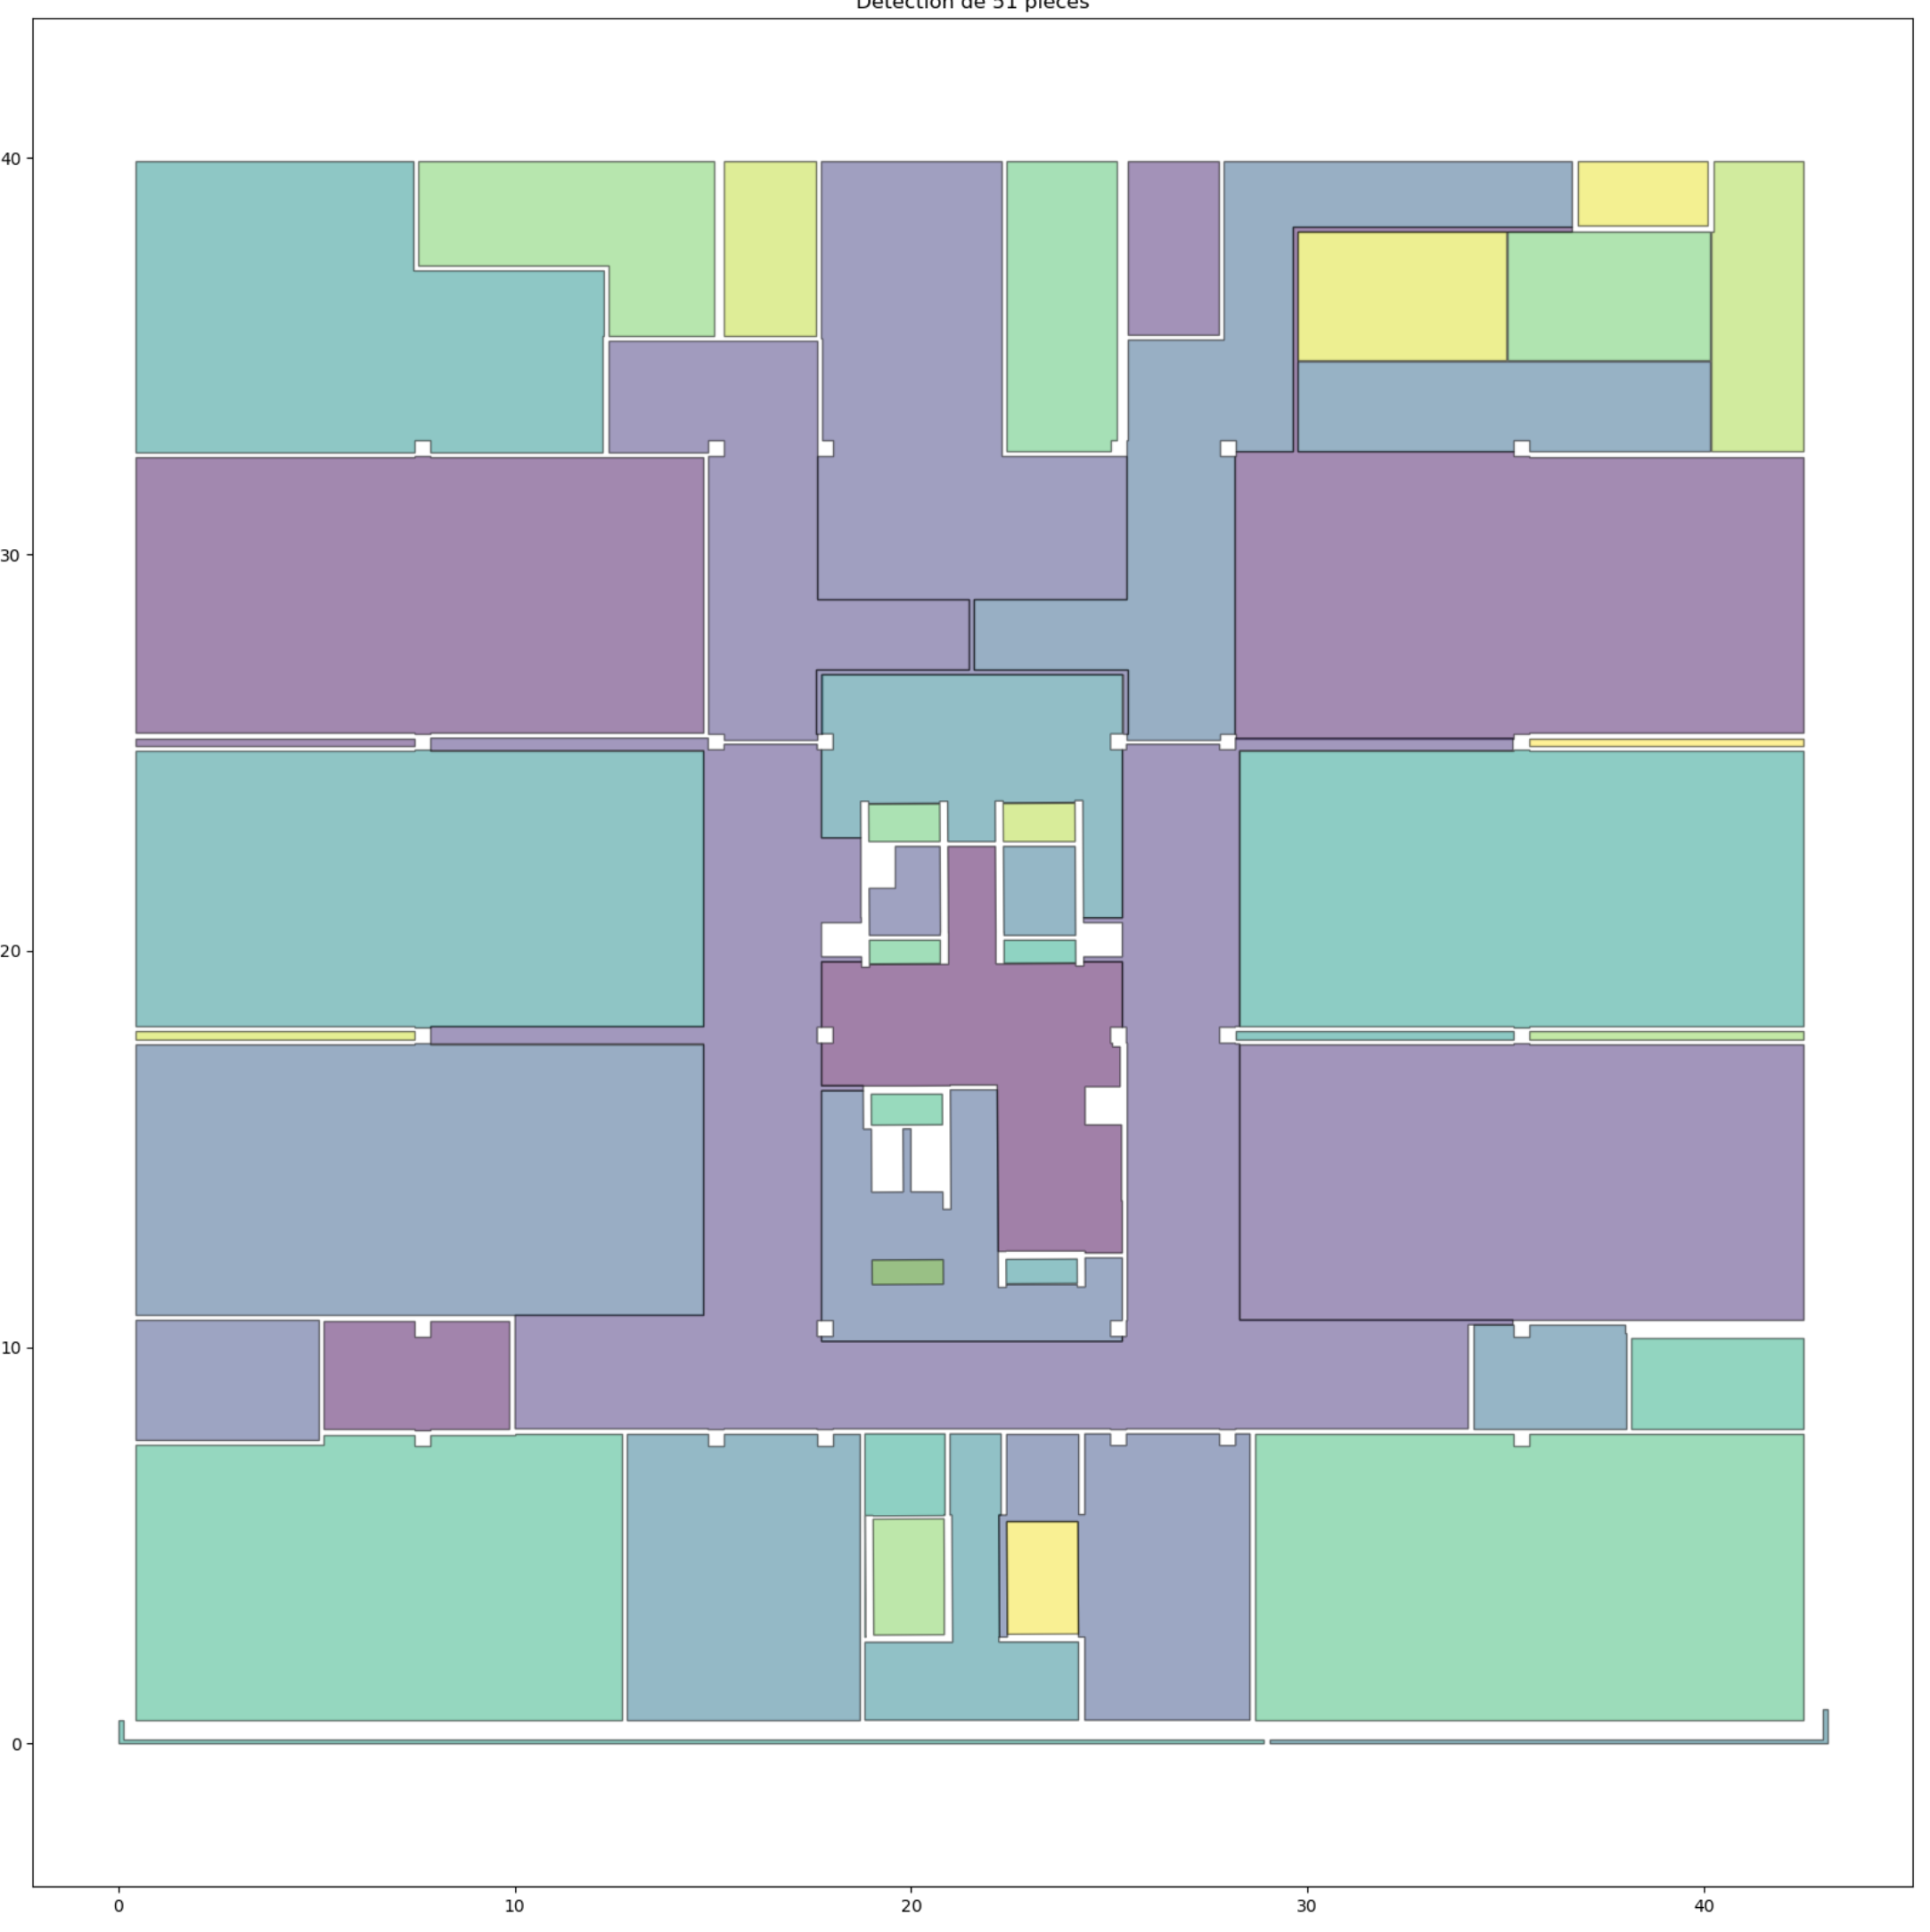
\includegraphics[width=0.3\linewidth]{figures/SBC_pred-1.png} \\
        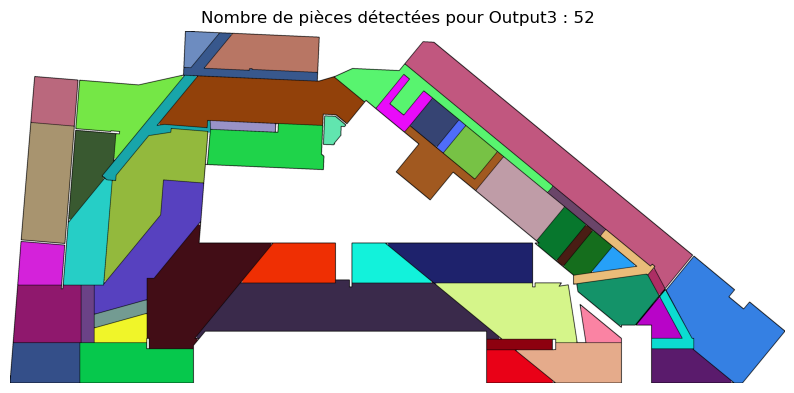
\includegraphics[width=0.3\linewidth]{figures/CVSeg_pred-3.png} &
        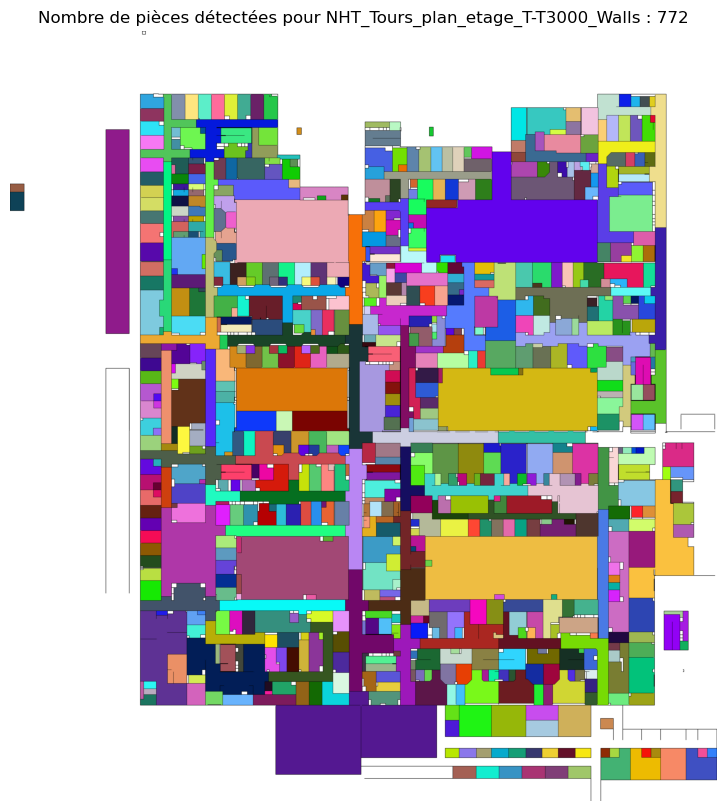
\includegraphics[width=0.3\linewidth]{figures/CVSeg_pred-2.png} &
        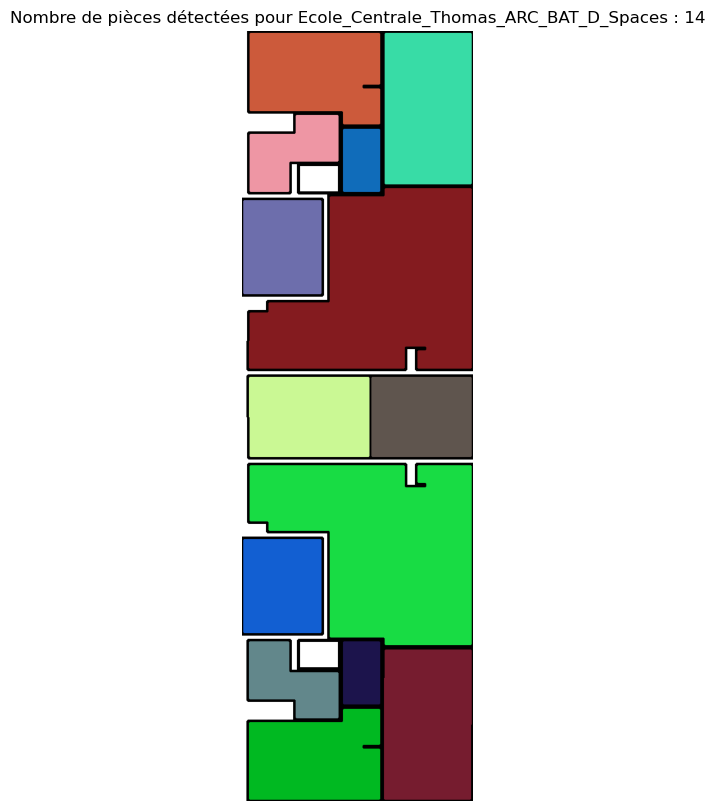
\includegraphics[width=0.3\linewidth]{figures/CVSeg_pred-1.png} \\
        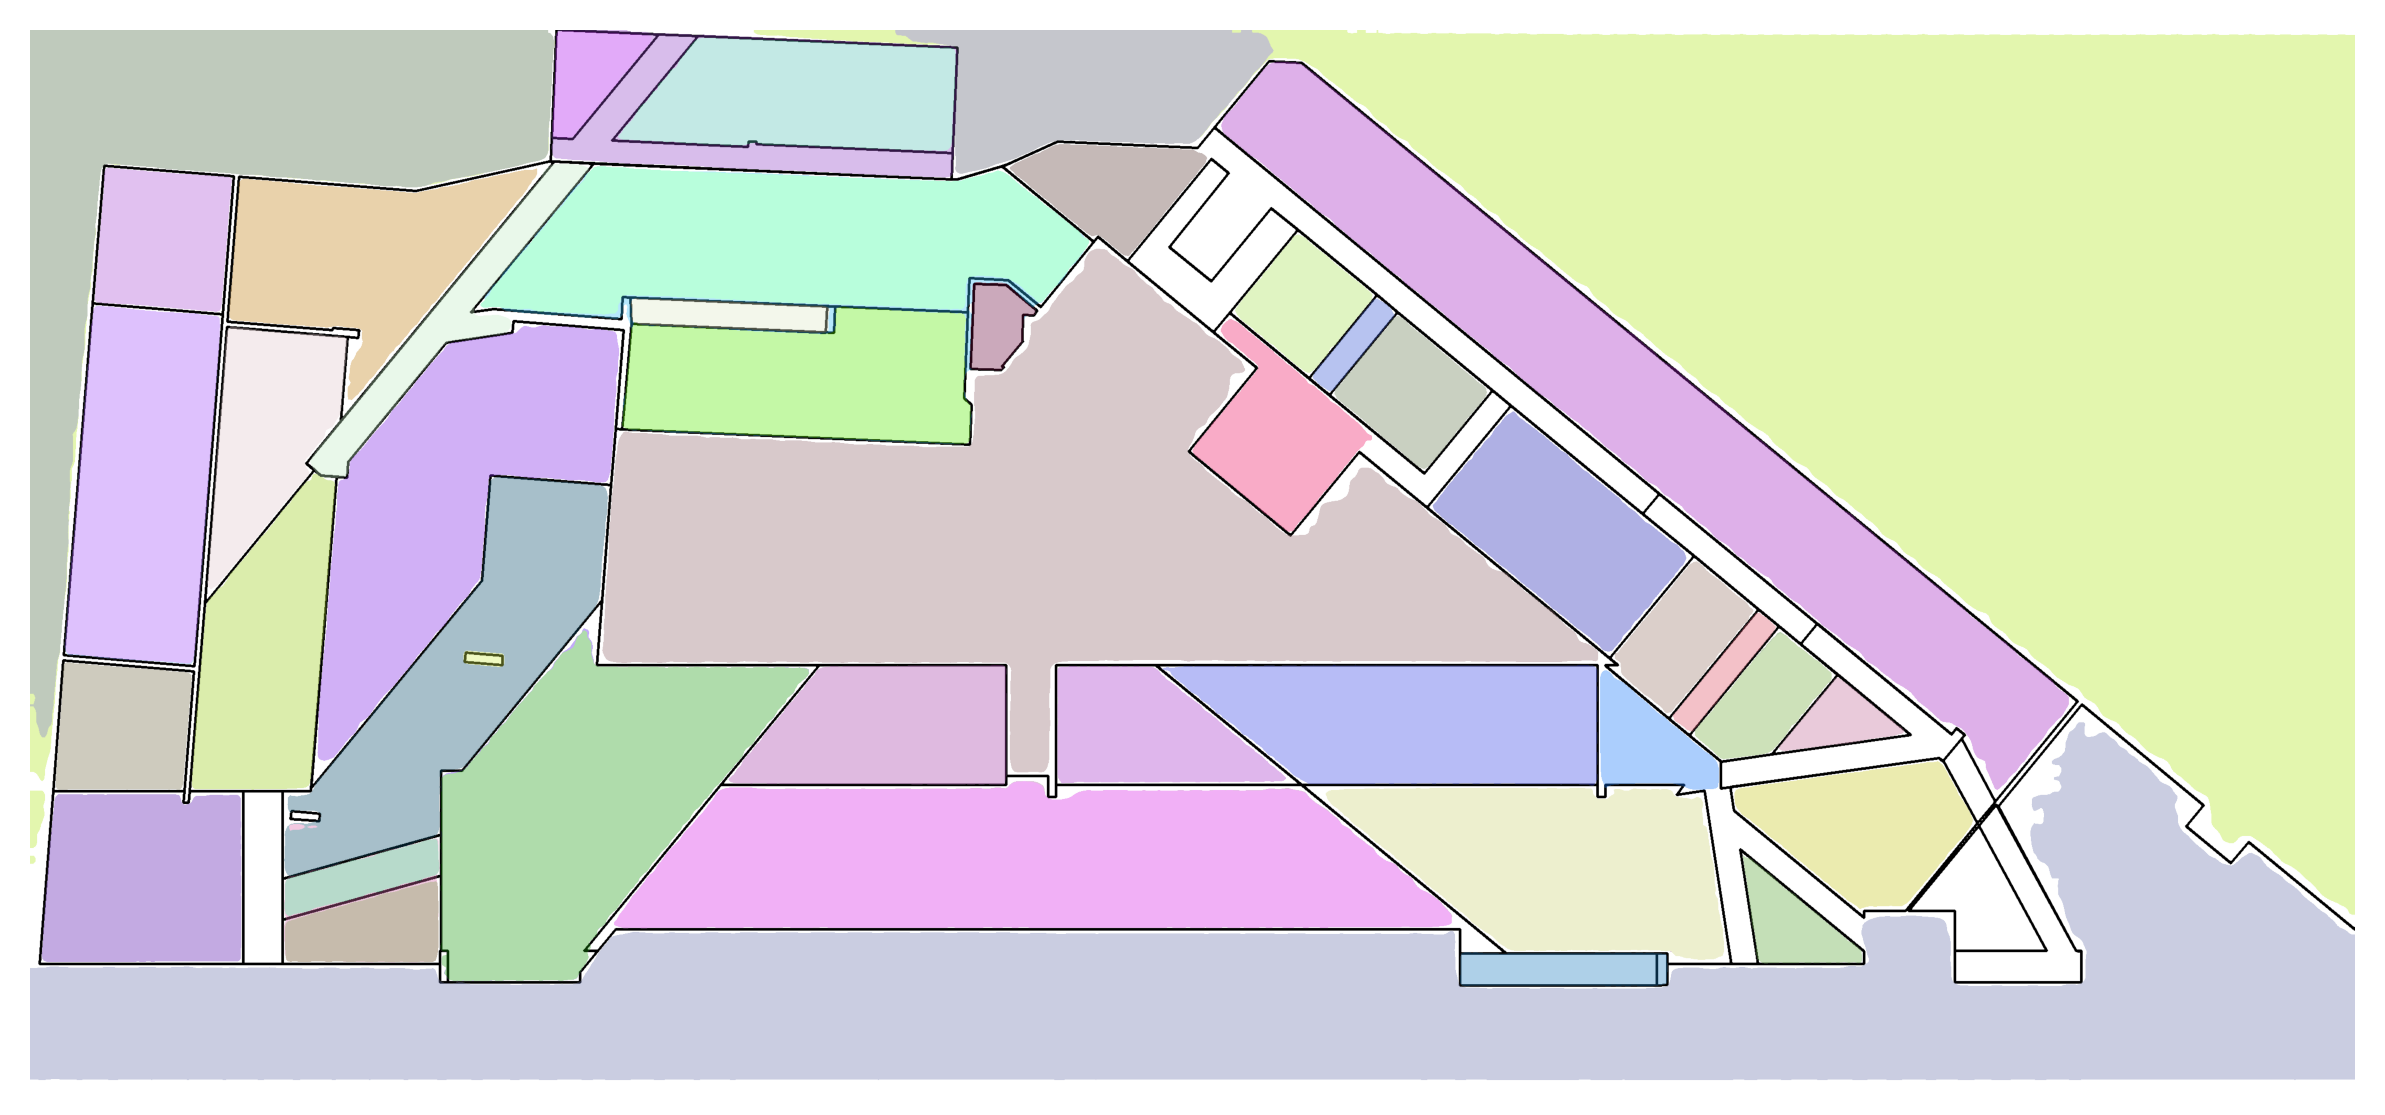
\includegraphics[width=0.3\linewidth]{figures/SAM_pred-1.png} &
        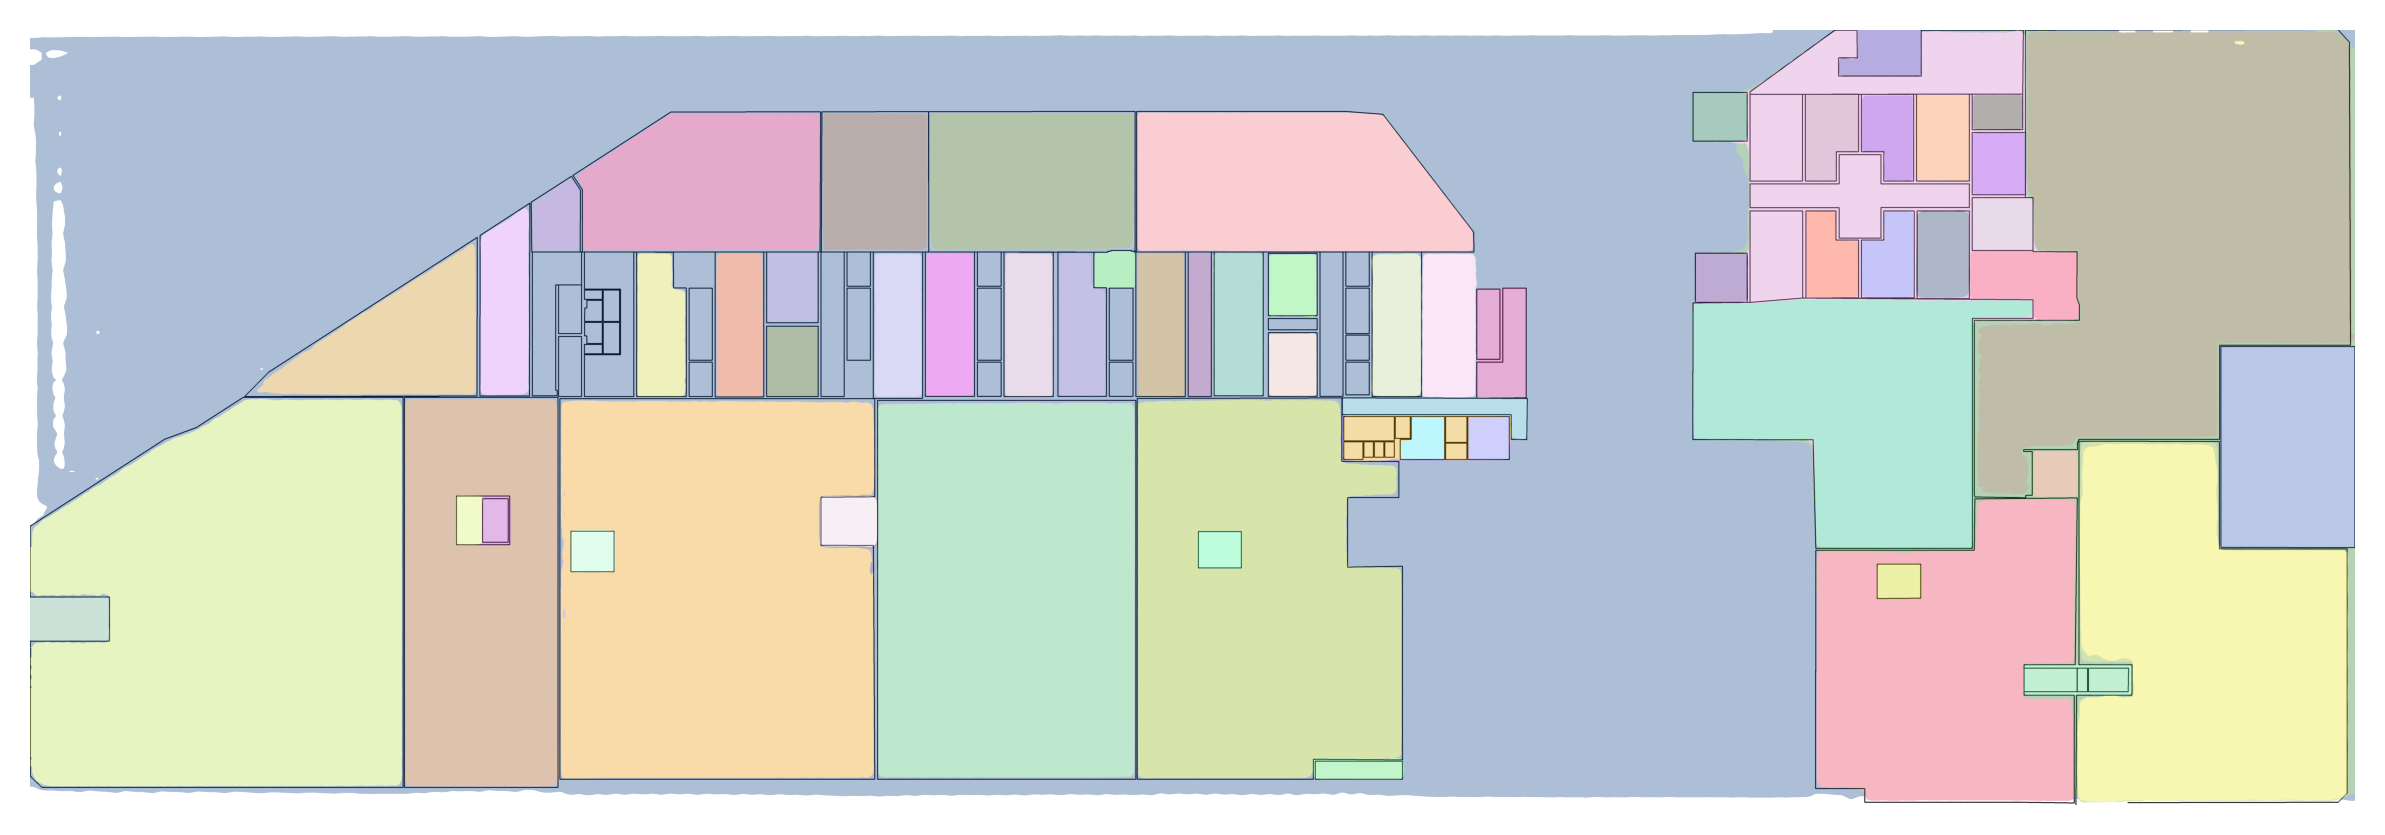
\includegraphics[width=0.3\linewidth]{figures/SAM_pred-2.png} &
        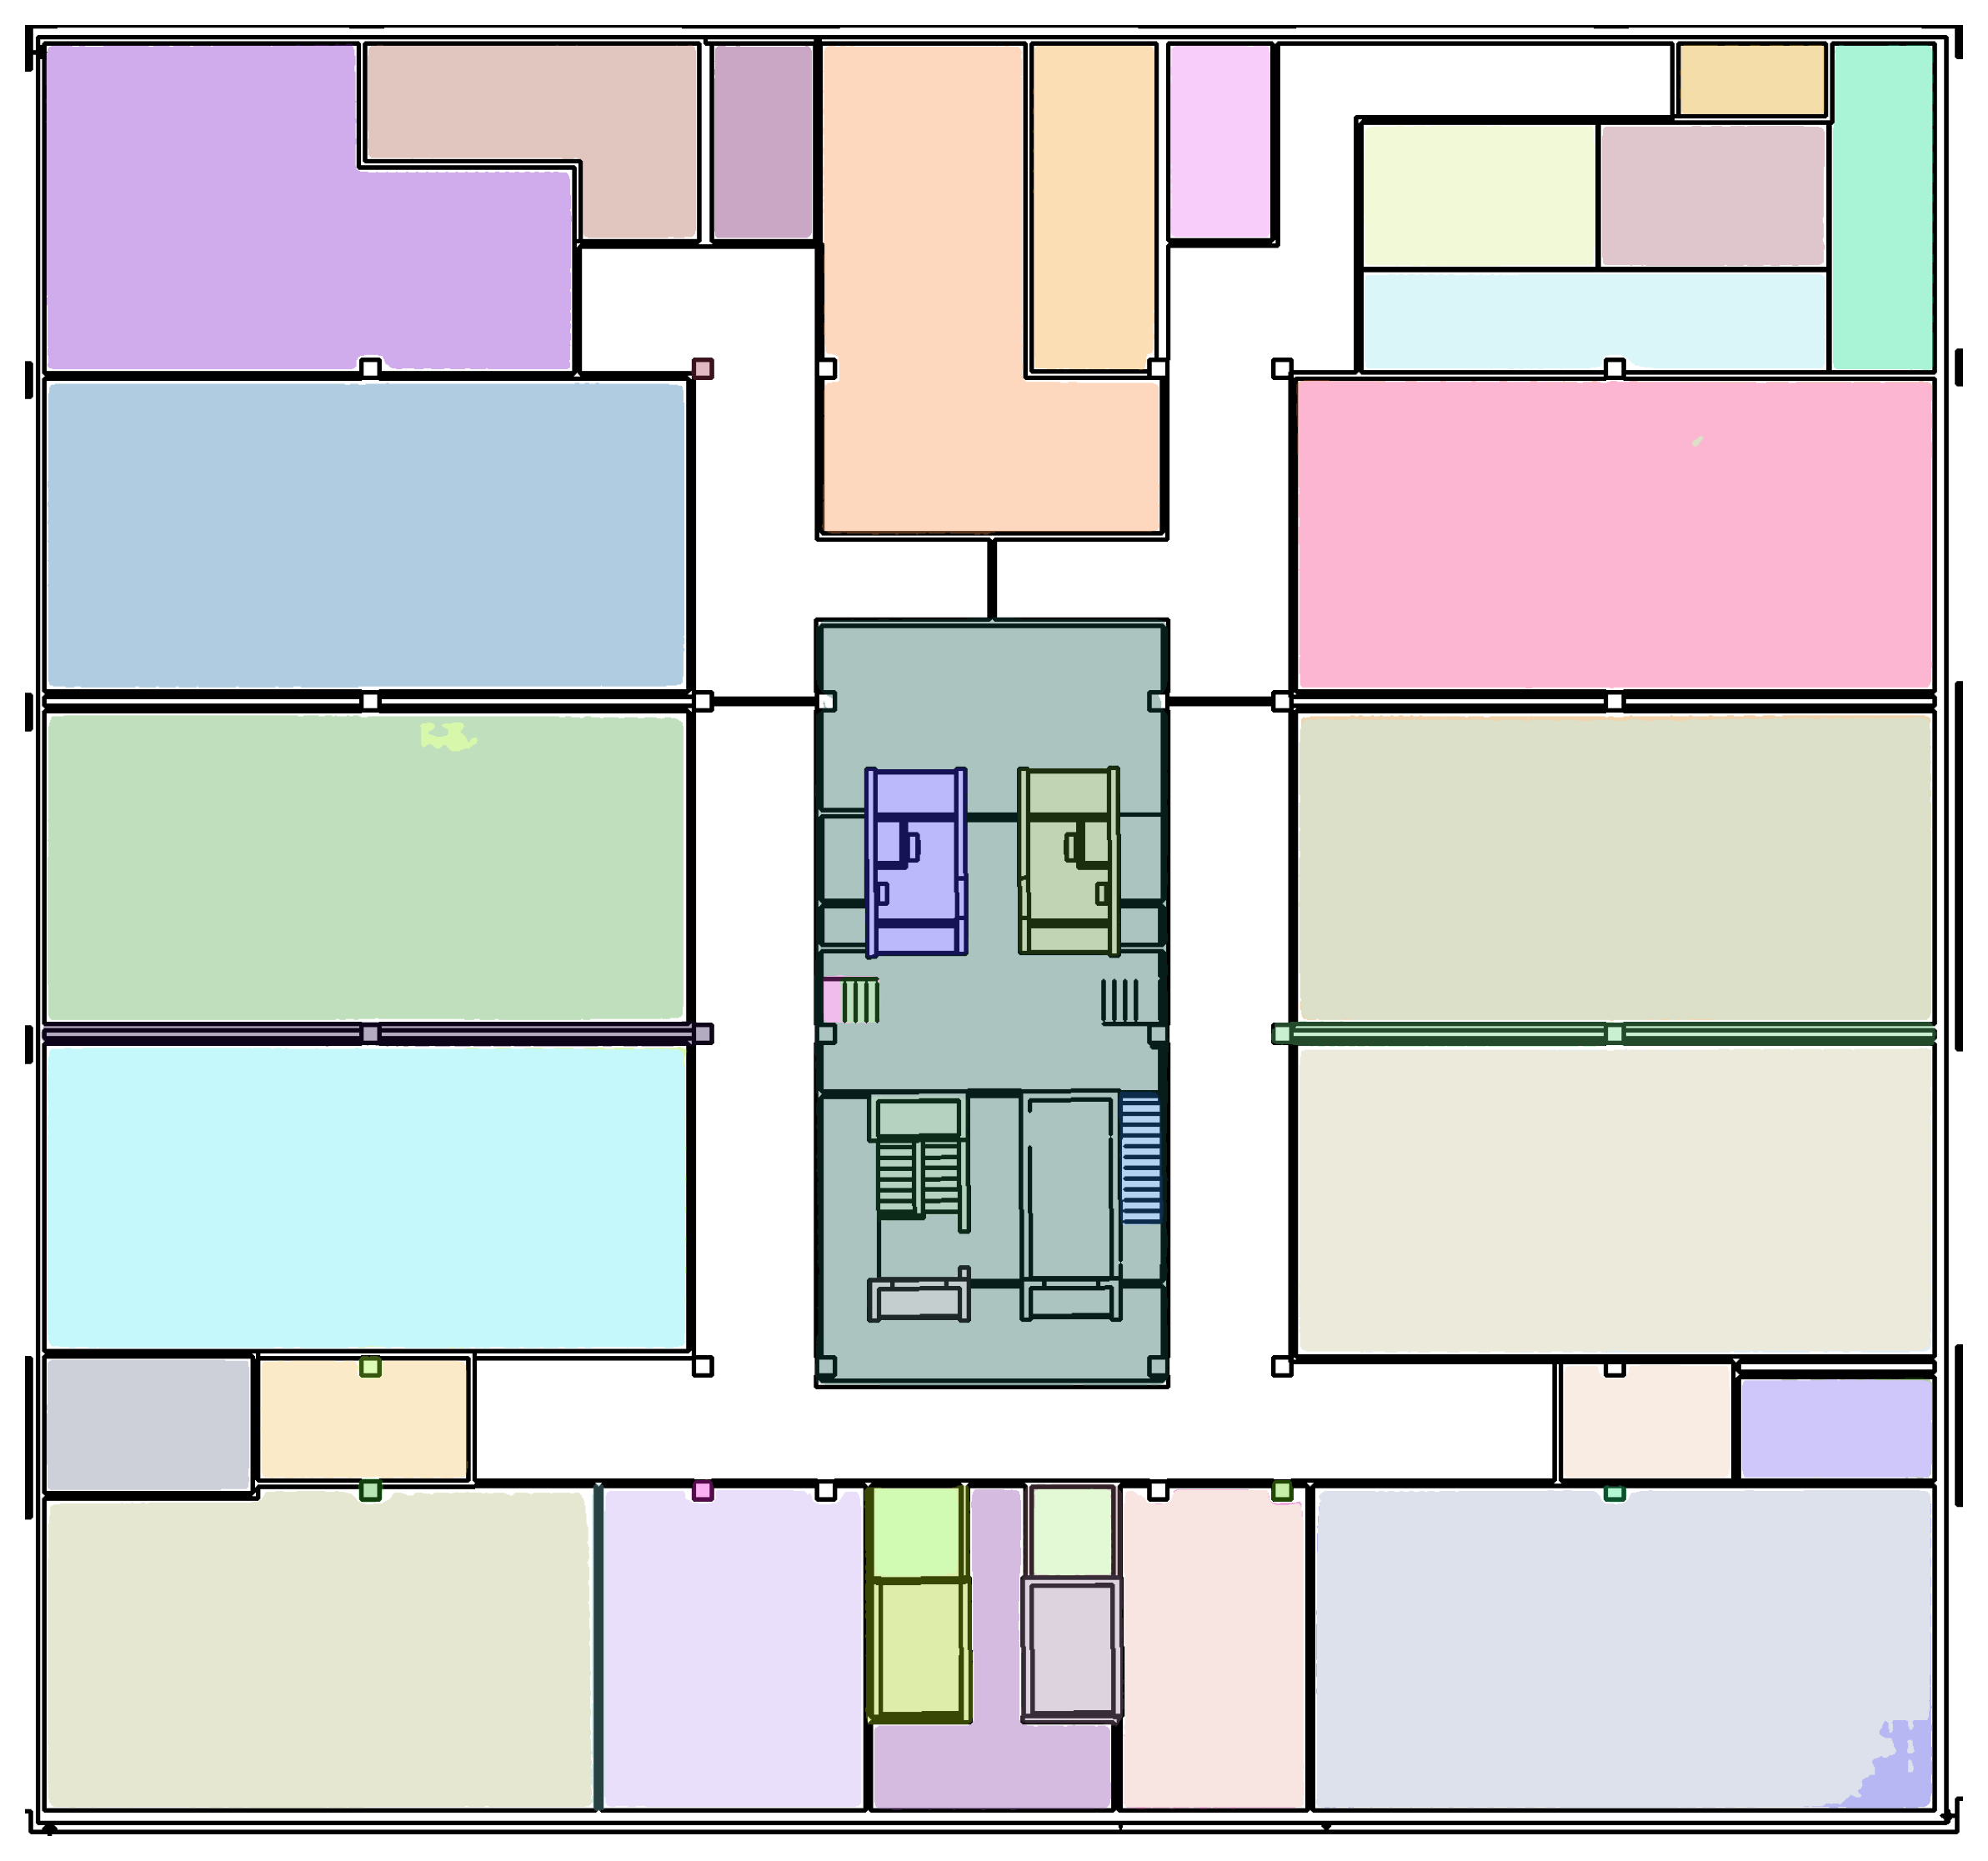
\includegraphics[width=0.3\linewidth]{figures/SAM_pred-3.png} \\
    \end{tabular}
    \caption{Segmentation outputs for random floor plans.
    First line: results of the \texttt{SegmentBasedClustering} model.
    Second line: results of the \texttt{VisionSegmentation} model.
    Third line: results of the \texttt{SegmentAnythingModel} model.}
    \label{fig:segmentation_results}
\end{figure}

% =============================================================================
% End of the document
% =============================================================================
\end{document}